\documentclass[a4paper,12pt]{article}

% ---------- Lingua e codifica ----------
\usepackage[utf8]{inputenc}    % Codifica UTF-8
\usepackage[T1]{fontenc}       % Codifica font
\usepackage[italian]{babel}    % Lingua italiana

% ---------- Font ----------
\usepackage{times}             % Times New Roman

% ---------- Layout pagina ----------
\usepackage{geometry}
\geometry{margin=2.5cm}        % Margini

% ---------- Grafica e immagini ----------
\usepackage{graphicx}
\usepackage{longtable}
\usepackage{float}

% ---------- tabelle più stabili con link ---------
\usepackage{tabularx}

% ---------- dockerfile ---------

\usepackage{listings}


% ------------------------ fancyhdr ------------------------
\usepackage{fancyhdr}
\pagestyle{fancy}

% Cancella intestazioni e piè di pagina predefiniti
\fancyhf{}

% Intestazione
\fancyhead[R]{\textcolor{gray}{\nouppercase{\leftmark}}} % nome della sezione/paragrafo corrente
%\fancyhead[C]{}         % centro (vuoto)
%\fancyhead[R]{}         % destra (vuoto)

% Piè di pagina
\fancyfoot[L]{\textcolor{gray}{Software Requirements Specifications - \textit{BugBoard26}} \hfill\thepage}
\fancyfoot[C]{}
\fancyfoot[R]{}



% ---------- Stile titoli ----------
\usepackage{titlesec}
\titleformat{\section}{\normalfont\Large\bfseries}{\thesection}{1em}{}
\titleformat{\subsection}{\normalfont\large\bfseries}{\thesubsection}{1em}{}
\titleformat{\subsubsection}{\normalfont\normalsize\bfseries}{\thesubsubsection}{1em}{}

% ---------- Spaziatura e interlinea ----------
\usepackage{setspace}
\onehalfspacing % interlinea 1.5



\usepackage{imakeidx}  % più moderno
\makeindex[title=Indice analitico, intoc]  % aggiunge il titolo e l'inserimento nel sommario

% per checkbox
\usepackage{amssymb} 

% ---------- Link e riferimenti ----------
%\usepackage[hidelinks]{hyperref} questo era per il classico tutto nero
% i due package sotto sono per impostare i link colorati
% Attenzione deve essere l'ultimo pacchetto!!!
\usepackage[x11names]{xcolor} % serve per i colori nuovi, come forestgreen
\usepackage[colorlinks=true,
            linkcolor=blue,
            citecolor=ForestGreen,
            urlcolor=DarkOrange3]{hyperref}


\title{\textbf{Software Requirements Specifications (SRS)} \\ {\Huge BugBoard26} \\ \large Ver. 1.0  }
\author{Gruppo di Progetto: ID25\\
\begin{minipage}[t]{0.45\textwidth}
\raggedright
Luca Santangelo\\
\textit{N86002450}\\
\end{minipage}
\hfill
\begin{minipage}[t]{0.45\textwidth}
\raggedleft
Manuel Montuori\\
\textit{N86001690}\\
\end{minipage}
}
\date{\today}

\begin{document}

\maketitle
\newpage
\hypersetup{linkcolor=black} % serve per impedire che si colorino i link del sommario
\tableofcontents
\hypersetup{linkcolor=blue} % serve per ripristinare i colori dei link
\newpage

\section{Introduzione}
\subsection{Scopo del documento}
Questo documento si rivolge a membri e amministratori dei team di sviluppo
di progetti software, oltre che a stakeholders esterni. Ha lo scopo di illustrare il funzionamento dell'applicativo al quale fa riferimento. Esso è una piattaforma di gestione di issue in progetti software.
La piattaforma consente ad utenti autenticati di segnalare problemi in un progetto, 
monitorarne lo stato, assegnarli a membri del team e tenere traccia delle attività di risoluzione. 
I membri del team di sviluppo sono i soli a dover utilizzare il software.
\subsection{Campo di applicazione del sistema}
Il sistema software in fase di sviluppo sarà indicato come System Under Development (SUD) o semplicemente come \textit{BugBoard26}.
\textit{BugBoard26} dovrà svolgere le seguenti funzionalità \index{Funzionalità}:
\begin{enumerate}
    \item Provvederà all'autenticazione \index{Autenticazione} dell'utente, consentendogli di accedere solo a quelle funzionalità che gli competono.
    \item Gestirà un sistema di registrazione accessibile ai soli amministratori.
    \item Tutti gli utenti autenticati potranno segnalare una issue.
    \item La piattaforma sarà provvista di una vista riepilogativa \index{Vista!Riepilogo issue} delle issue, con possibilità di filtrare, ordinare e ricercare.
    \item Il sistema permetterà ad utenti amministratori di assegnare \index{Issue!Assegnazione issue} issue ad un membro del team. 
    \item Durante la fase di assegnazione di una issue, il sistema suggerirà l'utenza con il \index{Vista!Workload} carico di lavoro più basso.
    \item Il sistema potrà inviare notifiche agli utenti.
    \item Il sistema genererà report mensili sull'attività del team.
    \item Il sistema permetterà agli amministratori di visualizzare
    \index{Vista!Report mensile} i report sul team.

\end{enumerate}
\subsection{Definizioni, sinonimi adottati e abbreviazioni}
\subsubsection{Definizioni (Glossario)}
\index{Glossario}
\begin{itemize}
    \item Allegare: aggiungere un'immagine ad una issue, affinchè sia inclusa e consultabile assieme ad essa.
    \item Amministratore: persona che gestisce il team. Può fare tutto ciò che può fare un utente con permessi aggiuntivi.
    \item Attore: rappresenta un'entità esterna che sta interagendo con il SUD.
    \item Bug: malfuznionamento tecnico del prodotto software.

    \item Issue: problema ad un software, viene segnalato da un utente e può essere di quattro tipologie: 
      \begin{itemize}
        \item Question: per richieste di chiarimenti.
        \item Bug: per segnalare malfunzionamento del sistema.
        \item Documentation: problemi relativi alla documentazione.
        \item Feature: richiesta o suggerimento di nuove funzionalità.
    \end{itemize}
    \item Metrica: le metriche a cui si fa riferimento in questo documento sono: Numero di issue segnalate, numero di issue gestite, 
    tempo di risoluzione medio.
    \item Mock-up: rappresentazione visiva di un'interfaccia grafica o di una schermata del sistema.
    \item Notifica: sistema con cui la piattaforma comunica ad utenti autenticati alcune informazioni.
    \item Priorità: parametro di una issue. Se inserita in una issue richiede che la sua risoluzione debba essere considerata prioritaria dal team di sviluppo. \index{Priorità}
    \item Report: visualizzazione che sintetizza dati o informazioni sulle attività svolte.
    \item Scenario: sequenza di eventi che descrive l'interazione tra attori e sistema in un caso d'uso specifico.
    \item Segretezza: garantisce che le informazioni, i dati sensibili e le risorse di un sistema siano accessibili esclusivamente agli utenti che dispongono dell'autorizzazione esplicita.
    \item Semplice: intuituvo abbastanza da permette di interagire con il software senza la necessità di supporto.
    \item Sicuro: soddisfa requisiti atti a proteggere l'accesso non autorizzato alle risorse e a garantire l'integrità dei dati.
    \item Stakeholders: persona che ha un interesse nel prodotto software.

    \item Stato: la condizine in un dato momento della issue. Lo stato può assumere i seguenti valori:
    \begin{itemize}
        \item Todo: è inteso come stato inziale di una issue, è il valore dello stato nel momento della creazione. 
        \item In Progress: è inteso come stato intermedio nella risoluzione di una issue. Lo stato è impostato a \textit{In Progress} quando è stato assegnato ad un utente che ci dovrà lavorare.
        \item Done: è inteso come stato finale. Lo stato è impostato a \textit{Done} quanto la issue è stata risolta.
    \end{itemize}
    \item System under development: riferimento al sistema software che si sta progettando.
    \item Utente autenticato: persona membro del team autenticata nel sistema.
    \item Utente generico: persona del team che non ha ancora effettuato l'accesso al sistema.
    \item Vista: La vista è l'insieme di informazioni accessibile per il ogni utente.
\end{itemize}
\subsubsection{Sinonimi adottati}
\begin{itemize}
    \item Utente, utente generico, membro del team.
    \item Lista, elenco
    \item Ospite, stakeholder esterno.
    \item Sistema software, applicativo software, prodotto software, sud, piattaforma. 
    \item Autenticazione, log in
\end{itemize}
\subsubsection{Abbreviazioni}
\begin{itemize}
    \item Admin: abbreviazione di utente amministratore
    \item SUD: System under development
\end{itemize}
\subsection{Riferimenti}
Il presente documento è stato redatto in conformità allo standard IEEE Std 830-1998. \index{IEEE Std 830-1998}
Per la definizione dettagliata dei casi d’uso si è fatto riferimento alle tabelle di Alistair Cockburn.\index{Cockburn}\\
Riferimenti bibliografici per la stesura del documento:
\begin{itemize}
    \item \textit{IEEE Std 830-1998 (Revision of IEEE Std 830-1993) – IEEE Recommended Practice for Software Requirements Specifications.}
    \item \textit{Cockburn, A. (2001). Writing Effective Use Cases. Addison-Wesley.}
\end{itemize}
\subsection{Panoramica del documento}
La restante parte di questo documento è suddivisa in due ulteriori capitoli che descrivono le caratteristiche funzionali di \textit{BugBoard26}.\\
Il capitolo immediatamente seguente: "Descrizione generale" è composto dai seguenti paragrafi.
\begin{longtable}{|p{5cm}|p{9cm}|}
\hline
Prospettiva del prodotto & Illustra l'ambito in cui \textit{BugBoard26} si va ad inquadrare e sarà utilizzato\\ \hline
Funzionalità del prodotto & Esplicita le funzioni implementate da \textit{BugBoard26} \\ \hline
Utenti e attori del sistema & Individuazione e caratterizzazione di tutti gli utenti (attori) del sistema \\ \hline
Vincoli generali e assunzioni & Indica ciò a cui deve essere vincolato il prodotto software \\ \hline
\end{longtable}
Nel terzo capitolo "Requisiti specifici" saranno dettagliate tutte le funzionalità che \textit{BugBoard26} realizza.
Questo capitolo è composto dai seguenti paragrafi.
\begin{longtable}{|p{5cm}|p{9cm}|}
\hline
Requisiti funzionali & Si scende ad un livello di maggior dettaglio nella descrizione delle funzioni del prodotto software.\\ \hline
Requisiti non funzionali & Esplicita i requisiti non funzionali del prodotto software \textit{BugBoard26} \\ \hline
Modellazione dei casi d’uso & Si modellano, tramite UseCase Diagram, tutti i casi d'uso del prodotto software. \\ \hline
Formalizzazione di casi d’uso significativi & Si scende ad un livello di maggiore dettagio nella descrizione dei casi d'uso
utilizzando le tabelle di Cockburn. \\ \hline
Prototipazione visuale & Si descriveranno visualmente le risposte del sistema nel suo utilizzo attraversando il flusso dei casi d'uso. \\ \hline
\end{longtable}

\newpage
\section{Descrizione generale}
\subsection{Prospettiva del prodotto}
Il sistema \textit{BugBoard26} è un prodotto software autonomo progettato per la gestione interna delle issue nei team di sviluppo software.
Non fa parte di un sistema più grande e funziona indipendentemente.\\
Tutti gli utenti devono autenticarsi prima di accedere alle funzionalità.

\subsection{Funzionalità del prodotto}
\textit{BugBoard26} deve fornire le funzionalità \index{Funzionalità} di seguito riportate, che per motivi di chiarezza sono state organizzate in categorie:
\begin{itemize}
    \item Categoria Autenticazione\index{Autenticazione} - \textit{BugBoard26} consente l'autenticazione dell'utente, consentedogli di accedere solo alle funzionalità che gli competono.
    \begin{itemize}
        \item \hyperref[sec:RE01]{Autenticazione:} \textit{BugBoard26} contente l'autenticazione dell'utente.
        \index{Autenticazione}
        \item \hyperref[sec:RE02]{Registrazione nuova utenza (Amministratore):} Un amministratore registra una nuova utenza.\index{Nuova utenza (Amministratore)} 
    \end{itemize}
    \item Categoria issue\index{Issue} - \textit{BugBoard26} gestisce la segnalazione e l'assegnazione di issue.
    \begin{itemize}
        \item \hyperref[sec:RE03]{Segnala issue:}\index{Issue!Segnalazione}\index{Issue!Filtra}\index{Issue!Ordina}\index{Issue!Ricerca} Un utente autenticato può segnalare una issue, della quale deve inserire un titolo e una descrizione. Può anche impostare una priorità e un tipo. \index{Priorità}
        \item \hyperref[sec:RE04]{Assegna issue:}\index{Assegna} Un amministratore può assegnare una issue ad un membro del team.
        \item{Suggerimento utente:} Il sistema mostra una lista di utenti ordinati per carico di lavoro crescente. Il primo della lista viene suggerito esplicitamente all'amministratore.
        \item \hyperref[sec:RE04]{Modifica stato issue:} Quando una issue viene assegnata ad un utente il sistema ne modifica lo stato.\index{Issue!Modifica} 
    \end{itemize}
    \item Categoria visualizzazioni\index{Vista} -  \textit{BugBoard26} permette di visualizzare informazioni su issue e membri del team.
    \begin{itemize}
        \item \hyperref[sec:RE05]{Visualizza issue:}\index{Vista!Riepilogo issue} gli utenti autenticati possono visualizzare la lista delle issue.
        \item \hyperref[sec:RE06]{Visualizza report team:}\index{Vista!Report mensile} Gli amministratori hanno accesso ai report mensili del team.
        \item \hyperref[sec:RE07]{Visualizza issue utente:}\index{Vista!Issue personali} Gli utenti autenticati possono visualizzare le issue assegnategli da un amministratore.
        \item{Visualizza notifiche:} \index{Vista!Notifiche} Il sistema fornisce una dashboard per la visualizzazione e gestione delle proprie notifiche.
    \end{itemize}
    \item Categoria Notifiche\index{Notifiche} -  \textit{BugBoard26}  gestisce l'invio di notifiche agli utenti.
    \begin{itemize}
        \item{Invio notifiche:}\index{Notifiche!Invio} Il sistema notifica un utente quando un amministratore gli assegna una nuova issue.
        \item{Lettura notifiche:} Un utente può segnare le proprie notifiche come lette o come non lette.
    \end{itemize}
\end{itemize}

\subsection{Utenti e attori del sistema} 
\label{sec:attori}
La seguente tabella definisce gli utenti principali del sistema, descrivendone il possibile utilizzo e la competenza tecnica richiesta. L'insieme risulta esaustivo, non è 
previsto, quindi, che utenti non specificati in questa sezione utilizzino il sistema. Per "competenze basilari di utilizzo di applicativi software" si intende 
una media familiarità con strumenti informatici di base. Non è prevista una curva di apprendimento sull'utilizzo di \textit{BugBoard26}.\\ 

\begin{tabularx}{\textwidth}{|X|X|X|}
\hline
\multicolumn{3}{|c|}{\textbf{Membro del team autenticato}} \\ \hline
\textbf{Descrizione} & \textbf{Esperienza e competenze tecniche} & \textbf{Principali interazioni con il sistema} \\ \hline
È un membro del team di sviluppo software. Può autenticarsi per segnalare nuove issue e visualizzarle & Conoscenza base del dominio del software. Competenze basilari di utilizzo di applicativi software. & Segnala issue; visualizzare riepilogo issue; 
visualizzare le issue che gli sono state assegnate; ricevere notifiche dal sistema \\ \hline
\end{tabularx}

\begin{tabularx}{\textwidth}{|X|X|X|}
\multicolumn{3}{|c|}{\textbf{Amministratore}} \\ \hline
\textbf{Descrizione} & \textbf{Esperienza e competenze tecniche} & \textbf{Principali interazioni con il sistema} \\ \hline
È un utente autenticato con privilegi estesi. Oltre alle funzionalità dell’utente, può creare nuove utenze, assegnare issue ai membri del team 
e visualizzare report mensili sui membri del team. & Conoscenza base del dominio del software. Competenze basilari di utilizzo di applicativi software. &
Tutte le interazioni di un membro del team; assegna issue; visualizza report mensili \\ \hline
\end{tabularx}

\begin{tabularx}{\textwidth}{|X|X|X|}
\multicolumn{3}{|c|}{\textbf{Membro del team non autenticato}} \\ \hline
\textbf{Descrizione} & \textbf{Esperienza e competenze tecniche} & \textbf{Principali interazioni con il sistema} \\ \hline
È un utente che non ha effettuato l'accesso al sistema & Competenze basilari di utilizzo di applicativi software. &
Effettuare il log in. \\ \hline
\end{tabularx}

\newpage
\section{Requisiti specifici}

\subsection{Requisiti funzionali}

\subsubsection{RE01 - Log in utente}\index{Autenticazione}
\label{sec:RE01}

\begin{tabular}{|c|c|c|}
\hline
\multicolumn{3}{|c|}{Utenti per funzionalità} \\ \hline
\textbf{Utente} & \textbf{Utente autenticato} & \textbf{Amministratore} \\ \hline
\checkmark &  &  \\
\hline
\end{tabular} \\

\begin{tabularx}{\textwidth}{p{5cm}|X}
Funzione & Gestione dell'autenticazione utente \\ \hline
Descrizione & Il sistema deve permettere agli utenti di accedere al sistema tramite email e password. Solo utenti con credenziali
valide possono accedere al sistema \\ \hline
Input & Email e password \\ \hline
Fonte & Interfaccia di autenticazione \\ \hline
Output & Accesso al sistema con vista personalizzata o messaggio di errore \\ \hline
Azione & Verifica la validità delle credenziali permettendo l'accesso all'utente \\ \hline
Precondizione & Utenza registrata \\ \hline
Effetti collaterali & Nessuno \\ \hline 
Use Case & \hyperref[sec:UC01]{Vedi Use Case relativo a RE01} \\
\end{tabularx}


\subsubsection{RE02 - Nuova utenza (Amministratore)}\index{Nuova utenza (Amministratore)}
\label{sec:RE02}

\begin{tabular}{|c|c|c|}
\hline
\multicolumn{3}{|c|}{Utenti per funzionalità} \\ \hline
\textbf{Utente} & \textbf{Utente autenticato} & \textbf{Amministratore} \\ \hline
 &  & \checkmark \\
\hline
\end{tabular} \\

\begin{tabularx}{\textwidth}{p{5cm}|X}
Funzione & Registrazione nuova utenza \\ \hline
Descrizione & Il sistema deve permettere di registrare nuove utenze all'interno del sistema software. \\ \hline
Input & Email e ruolo \\ \hline
Fonte & Interfaccia con vista dedicata agli utenti amministratori \\ \hline
Output & Visualizza messaggio di avvenuta registrazione della nuova utenza o visualizza messaggio di errore \\ \hline
Azione & Attivazione della nuova utenza con possibilità di autenticazione \\ \hline
Richiede & Credenziali conformi alle regole imposte dal sistema software \\ \hline
Precondizione & L'utente deve essere autenticato con permessi di amministratore \\ \hline
Effetti collaterali & Il sistema inserisce un nuovo utente con credenziali riservate nel sistema \\ \hline 
Use Case & \hyperref[sec:UC01]{Vedi Use Case relativo a RE02} \\ \hline
\end{tabularx}




\subsubsection{RE03 - Segnala issue}\index{Issue!Segnalazione}
\label{sec:RE03}

\begin{tabular}{|c|c|c|}
\hline
\multicolumn{3}{|c|}{Utenti per funzionalità} \\ \hline
\textbf{Utente} & \textbf{Utente autenticato} & \textbf{Amministratore} \\ \hline
 & \checkmark & \checkmark \\
\hline
\end{tabular} \\

\begin{tabularx}{\textwidth}{p{5cm}|X}
Funzione & Segnalazione di una nuova issue \\ \hline
Descrizione & Il sistema deve permettere ad un utente di segnalare una nuova issue, specificando titolo, descrizione e, eventualmente, 
impostare un tipo e una priorità. Tipo: \index{Priorità}
\begin{itemize}
    \item Bug
    \item Documentation
    \item Feature
    \item Question
\end{itemize}. Priorità: 
\begin{itemize}
    \item High
    \item Medium
    \item Low
\end{itemize}. \\ \hline
Input & Titolo, descrizione e opzionalmente tipo e priorità \\ \hline
Fonte & Interfaccia utente di segnalazione issue \\ \hline
Output & Visualizza un messaggio di avventua segnalazione della nuova issue o un messaggio di errore \\ \hline
Azione & Il sistema crea la nuova issue \\ \hline
Richiede & Titolo e descrizione \\ \hline
Precondizione & L'utente deve essere autenticato \\ \hline
Effetti collaterali & Il sistema impostato lo stato della nuova issue a \textit{Todo}. \\ \hline 
Use Case & \hyperref[sec:UC02]{Vedi Use Case relativo a RE03} \\ \hline
Descrizione dettagliata Cockburn & \hyperref[sec:CKB01]{Vedi la descrizione dettagliata con le tabelle di Cockburn} \\ \hline
\end{tabularx}

\subsubsection{RE04 - Assegna issue}\index{Issue!Assegnazione}
\label{sec:RE04}

\begin{tabular}{|c|c|c|}
\hline
\multicolumn{3}{|c|}{Utenti per funzionalità} \\ \hline
\textbf{Utente} & \textbf{Utente autenticato} & \textbf{Amministratore} \\ \hline
 & & \checkmark \\
\hline
\end{tabular} \\

\begin{tabularx}{\textwidth}{p{5cm}|X}
Funzione & Assegnazione di una issue ad un membro del team registrato nel sistema \\ \hline
Descrizione & Il sistema deve permettere di assegnare issue a membri del team e modificare lo stato della issue da Todo a In progress. Stato: 
\begin{itemize}
    \item Todo
    \item In progress
    \item Done
\end{itemize} \\ \hline
Input & Identificativo issue e Identificativo utente a cui è assegnata la issue \\ \hline
Fonte & Interfaccia utente di assegnazione issue \\ \hline
Output & Visualizza messaggio di avventa assegnazione della issue o messaggio di errore \\ \hline
Azione & Il sistema deve assegnare la issue all'utente segnalato \\ \hline
Precondizione & L'utente deve essere autenticato con permessi di amministratore. \\ \hline
Effetti collaterali & Il sistema invia una notifica all'utente cui è stata assegnata la issue e modifica lo 
stato della issue da \textit{Todo} a \textit{In Progress}. \\ \hline 
Use Case & \hyperref[sec:UC03]{Vedi Use Case relativo a RE04} \\ \hline
\end{tabularx}


\subsubsection{RE05 - Visualizza riepilogo issue}\index{Vista!Riepilogo issue}
\label{sec:RE05}

\begin{tabular}{|c|c|c|}
\hline
\multicolumn{3}{|c|}{Utenti per funzionalità} \\ \hline
\textbf{Utente} & \textbf{Utente autenticato} & \textbf{Amministratore} \\ \hline
 & \checkmark & \checkmark \\
\hline
\end{tabular} \\

\begin{tabularx}{\textwidth}{p{5cm}|X}
Funzione & Visualizzazione del riepilogo delle issue \\ \hline
Descrizione & Il sistema deve permettere la visualizzazione di tutte le issue \\ \hline
Input & Richiesta di visualizzazione dell'elenco delle issue \\ \hline
Fonte & Interfaccia utente \\ \hline
Output & Elenco di tutte le issue presenti nel sistema \\ \hline
Azione & Il sistema deve gestire la visualizzazione delle issue presenti nel sistema \\ \hline
Precondizione & L'utente deve essere autenticato \\ \hline
Effetti collaterali & Nessuno \\ \hline 
Use Case & \hyperref[sec:UC04]{Vedi Use Case relativo a RE05} \\ \hline
\end{tabularx}


\subsubsection{RE06 - Visualizza report team}\index{Vista!Report mensile}
\label{sec:RE06}

\begin{tabular}{|c|c|c|}
\hline
\multicolumn{3}{|c|}{Utenti per funzionalità} \\ \hline
\textbf{Utente} & \textbf{Utente autenticato} & \textbf{Amministratore} \\ \hline
 & & \checkmark \\
\hline
\end{tabular} \\


\begin{tabularx}{\textwidth}{p{5cm}|X}

Funzione & Visualizzazione del report mensile del team \\ \hline
Descrizione & Il sistema deve permettere la visualizzazione di metriche aggregate e dettagliate per ogni singolo utente \\ \hline
Input & Mese richiesto \\ \hline
Fonte & Interfaccia utente amministratore \\ \hline
Output & Elenco del report mensile \\ \hline
Azione & Il sistema deve visualizzare il report \\ \hline
Precondizione & L'utente deve essere autenticato con permessi di amministratore \\ \hline
Effetti collaterali & Nessuno \\ \hline 
Use Case & \hyperref[sec:UC04]{Vedi Use Case relativo a RE06} \\ \hline
\end{tabularx}

\subsubsection{RE07 - Utente visualizza le proprie issue assegnate}\index{Vista!Issue personali}
\label{sec:RE07}

\begin{tabular}{|c|c|c|}
\hline
\multicolumn{3}{|c|}{Utenti per funzionalità} \\ \hline
\textbf{Utente} & \textbf{Utente autenticato} & \textbf{Amministratore} \\ \hline
 & \checkmark & \checkmark \\
\hline
\end{tabular} \\

\begin{tabularx}{\textwidth}{p{5cm}|X}
Funzione & Visualizzazione delle issue assegnate ad un utente \\ \hline
Descrizione & Il sistema deve permettere la visualizzazione ad un utente delle issue che gli sono state assegnate \\ \hline
Input & Richiesta di visualizzazione \\ \hline
Fonte & Interfaccia utente \\ \hline
Output & Elenco delle issue \\ \hline
Azione & Il sistema deve permettere la visualizzazione l'elenco \\ \hline
Precondizione & L'utente deve essere autenticato \\ \hline
Effetti collaterali & Nessuno \\ \hline
Use Case & \hyperref[sec:UC03]{Vedi Use Case relativo a RE07} \\ \hline
\end{tabularx}


\subsubsection{RE08 - Filtra issue}\index{Issue!Filtra}
\label{sec:RE08}

\begin{tabular}{|c|c|c|}
\hline
\multicolumn{3}{|c|}{Utenti per funzionalità} \\ \hline
\textbf{Utente} & \textbf{Utente autenticato} & \textbf{Amministratore} \\ \hline
  & \checkmark & \checkmark \\
\hline
\end{tabular} \\

\begin{tabularx}{\textwidth}{p{5cm}|X}
Funzione & Filtraggio delle issue \\ \hline
Descrizione & Il sistema deve permettere all'utente che intende visualizzare le issue di
applicare un filtro in base ai seguenti criteri:
\begin{itemize}
    \item Tipologia
    \item Priorità \index{Priorità}
    \item Stato
\end{itemize}
\\ \hline
Input & Seleziona il criterio \\ \hline
Fonte & Interfaccia utente nella vista di visualizzazione delle issue \\ \hline
Output & Elenco delle issue filtrate \\ \hline
Azione & Il sistema deve applicare il filtro e aggiornare l'elenco delle issue \\ \hline
Precondizione & L'utente deve essere autenticato e deve esistere almeno una issue nel sistema \\ \hline
Effetti collaterali & Nessuno \\ \hline
Use Case & Incluso in \hyperref[sec:UC04]{Visualizza riepilogo issue - RE05} \\ \hline
\end{tabularx}

\subsubsection{RE09 - Ordina issue}\index{Issue!Ordine}
\label{sec:RE09}

\begin{tabular}{|c|c|c|}
\hline
\multicolumn{3}{|c|}{Utenti per funzionalità} \\ \hline
\textbf{Utente} & \textbf{Utente autenticato} & \textbf{Amministratore} \\ \hline
 & \checkmark & \checkmark \\
\hline
\end{tabular} \\

\begin{tabularx}{\textwidth}{p{5cm}|X}
Funzione & Ordinamento delle issue \\ \hline
Descrizione & Il sistema deve permettere all'utente di ordinare le issue visualizzate secondo i seguenti criteri:
\begin{itemize}
    \item Titolo
    \item Descrizione
    \item Tipologia
    \item Priorità \index{Priorità}
    \item Stato
    \item Data di creazione
    \item Data di risoluzione
\end{itemize}
\\ \hline
Input & Seleziona il criterio di ordinamento \\ \hline
Fonte & Interfaccia utente nella vista di visualizzazione delle issue \\ \hline
Output & Elenco delle issue ordinate \\ \hline
Azione & Il sistema deve mostrare l'elenco delle issue ordinate \\ \hline
Precondizione & L'utente deve essere autenticato e deve esistere almeno una issue nel sistema \\ \hline
Effetti collaterali & Nessuno \\ \hline
Use Case & Incluso in \hyperref[sec:UC04]{Visualizza riepilogo issue - RE05} \\ \hline
\end{tabularx}

\subsubsection{RE010 - Ricerca issue}\index{Issue!Ricerca}
\label{sec:RE10}

\begin{tabular}{|c|c|c|}
\hline
\multicolumn{3}{|c|}{Utenti per funzionalità} \\ \hline
\textbf{Utente} & \textbf{Utente autenticato} & \textbf{Amministratore} \\ \hline
 & \checkmark & \checkmark \\
\hline
\end{tabular} \\

\begin{tabularx}{\textwidth}{p{5cm}|X}
Funzione & Ricerca delle issue \\ \hline
Descrizione & Il sistema deve permettere all'utente di effettuare una ricerca delle issue secondo i seguenti criteri: 
\begin{itemize}
    \item Titolo
    \item Descrizione
\end{itemize}
\\ \hline
Input & Chiave di ricerca \\ \hline
Fonte & Interfaccia utente nella vista di visualizzazione delle issue \\ \hline
Output & Elenco delle issue trovate \\ \hline
Azione & Il sistema deve mostrare l'elenco delle issue ritenute pertinenti con la ricerca \\ \hline
Precondizione & L'utente deve essere autenticato. \\ \hline
Effetti collaterali & Nessuno \\ \hline
Use Case & Incluso in \hyperref[sec:UC04]{Visualizza riepilogo issue - RE05} \\ \hline
\end{tabularx}

\subsubsection{RE011 - Visualizza notifiche}\index{Vista!Notifiche}
\label{sec:RE11}

\begin{tabular}{|c|c|c|}
\hline
\multicolumn{3}{|c|}{Utenti per funzionalità} \\ \hline
\textbf{Utente} & \textbf{Utente autenticato} & \textbf{Amministratore} \\ \hline
 & \checkmark & \checkmark \\
\hline
\end{tabular} \\

\begin{tabularx}{\textwidth}{p{5cm}|X}
Funzione & Visualizzazione elenco notifiche \\ \hline
Descrizione & Il sistema permette la visualizzazione dell'elenco di tutte le notifiche inviate all'utente autenticato. Con visualizzazione specifica tra notifiche lette e non lette. \\ \hline
Input & Seleziona pagina di notifiche \\ \hline
Fonte & Interfaccia utente nella vista di visualizzazione delle notifiche \\ \hline
Output & Elenco delle notifiche \\ \hline
Azione & Il sistema deve mostrare l'elenco delle notifiche \\ \hline
Precondizione & L'utente deve essere autenticato. \\ \hline
Effetti collaterali & Nessuno \\ \hline
Use Case & Incluso in \hyperref[sec:UC06]{Visualizza elenco notifiche - RE11} \\ \hline
\end{tabularx}

\subsubsection{RE012 - Lettura notifiche}\index{Notifiche!Lettura notifiche}
\label{sec:RE12}

\begin{tabular}{|c|c|c|}
\hline
\multicolumn{3}{|c|}{Utenti per funzionalità} \\ \hline
\textbf{Utente} & \textbf{Utente autenticato} & \textbf{Amministratore} \\ \hline
 & \checkmark & \checkmark \\
\hline
\end{tabular} \\

\begin{tabularx}{\textwidth}{p{5cm}|X}
Funzione & Una notifica può essere impostata come letta \\ \hline
Descrizione & Il sistema permette all'utente di impostare una notifica come letta o come non letta in qualsiasi momento. \\ \hline
Input & Seleziona tasto "segna come letto" o "segna come non letto" \\ \hline
Fonte & Interfaccia utente nella vista di visualizzazione delle notifiche \\ \hline
Output & Parametro di lettura modificato \\ \hline
Azione & Il sistema deve mostrare l'elenco aggiornato delle notifiche con i realitivi parametri di lettura\\ \hline
Precondizione & L'utente deve essere autenticato. \\ \hline
Effetti collaterali & Nessuno \\ \hline
Use Case &  \\ \hline
\end{tabularx}

\subsubsection{RE013 - Workload}\index{Workload}
\label{sec:RE13}

\begin{tabular}{|c|c|c|}
\hline
\multicolumn{3}{|c|}{Utenti per funzionalità} \\ \hline
\textbf{Utente} & \textbf{Utente autenticato} & \textbf{Amministratore} \\ \hline
 & & \checkmark \\
\hline
\end{tabular} \\

\begin{tabularx}{\textwidth}{p{5cm}|X}
Funzione & Il sistema suggerisce l'utente con il carico di lavoro più basso \\ \hline
Descrizione & Il sistema permette all'amministratore di scegliere l'utente a cui assegnare la issue in una lista di utenti ordinata per carico di lavoro crescente. \\ \hline
Input & Assegna issue \\ \hline
Fonte & Interfaccia utente nella assegnazione di una issue \\ \hline
Output & Lista ordinata di utenti per carico di lavoro \\ \hline
Azione & Il sistema deve mostrare l'elenco degli utenti ordinata in base al carico di lavoro in ordine crescente \\ \hline
Precondizione & L'utente deve essere autenticato come amministratore. \\ \hline
Effetti collaterali & Nessuno \\ \hline
Use Case &  \\ \hline
\end{tabularx}

\subsection{Modellazione dei casi d'uso tramite Use Case Diagram}

\subsubsection{Use Case Diagram}\index{Use Case}
\label{sec:UCD}
Di seguito è riportato il diagramma dei casi d’uso del System Under Development. Le prossime sezioni del documento  (3.3.1 - 3.3.5) presenteranno 
alcuni Use Case Diagram parziali, estratti dal diagramma complessivo, con l’unico scopo di facilitare la lettura e la comprensione 
dei singoli casi d’uso.
\begin{figure}[H]
    \centering
    
\includegraphics[width=1.0\textwidth]{images/BugBoard26.jpg}
    \caption{Use Case Diagram}
    \label{fig:etichetta}
\end{figure}


\subsubsection{Use Case Diagram parziale 1}\index{Use Case!Autenticazione}
\label{sec:UC01}
Il seguente Use Case è un estratto dello Use Case generale. Non aggiunge informazioni al caso d'uso specifico. Serve solamente a focalizzare l'attenzione sul caso/i d'uso specifico/i.
I casi d'uso mostrati sono due: \textit{Log in e Registra nuova utenza}. 
\begin{itemize}
    \item \textit{Log in}. L'attore principale è un Utente, esso può effettuare un Log in per autenticarsi nel sistema ed 
avere accesso alle funzionalità garantite dai privilegi della sua utenza. Per effettuare il Log in necessita di una email e una password corrispondenti ad un utente 
registrato e attivo nel sistema. 
    \item \textit{Registra nuova utenza}. L'attore principale è un amministratore. Esso può registrare nuove utenze nel sistema
specificando una email il ruolo. 
\end{itemize} 
\begin{figure}[H]
    \centering
    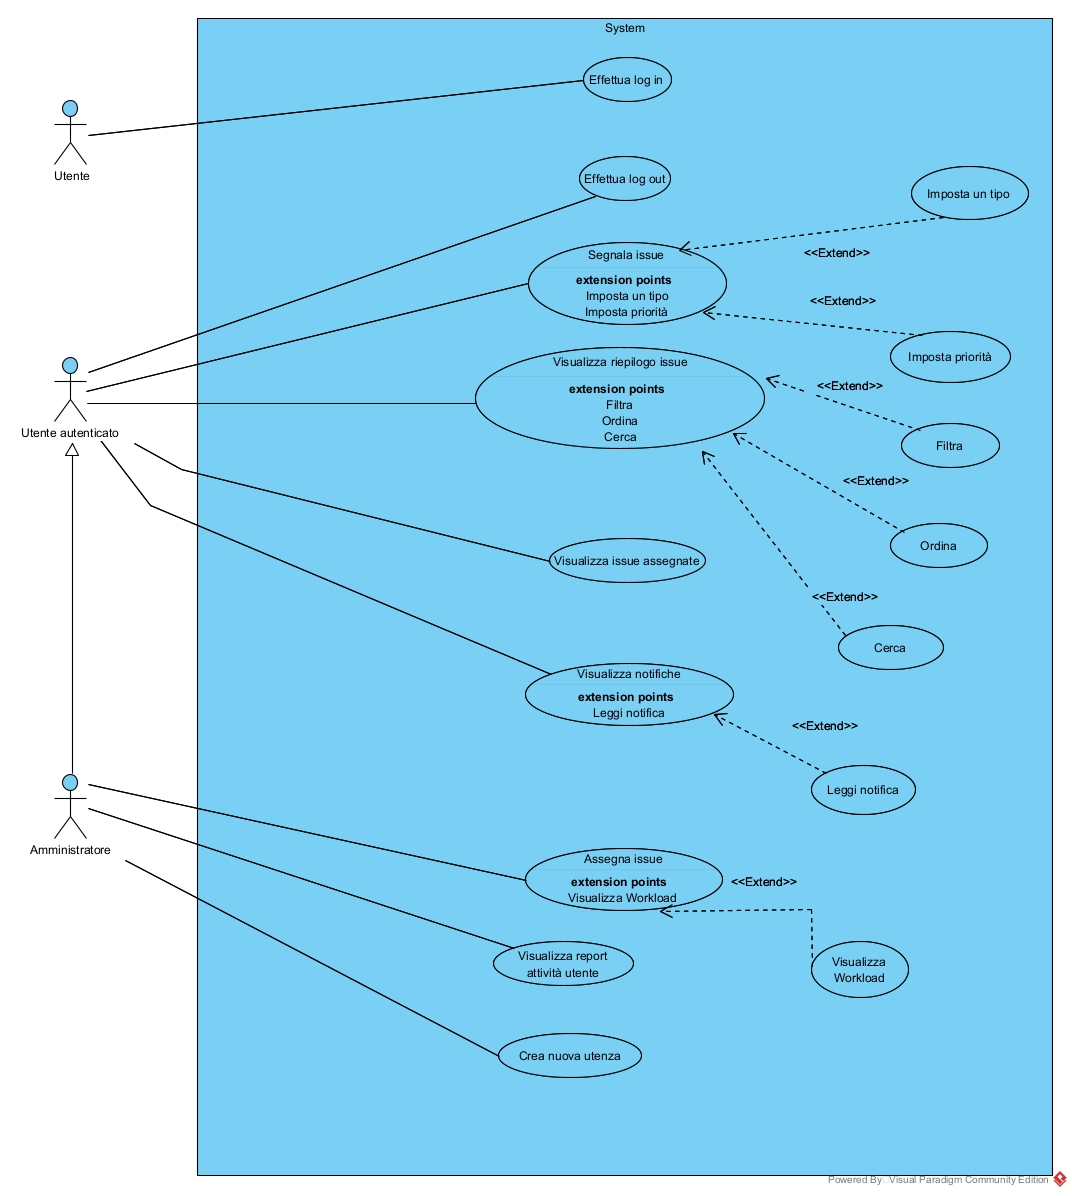
\includegraphics[width=0.8\textwidth]{images/Parziali/BugBoard26_login.jpg}
    \caption{Use Case1 - \hyperref[sec:RE01]{Requisito funzionale 3.1.1 - Log in utente} e \hyperref[sec:RE02]{Requisito funzionale 3.1.2 -  Crea nuova utenza}}
    \label{fig:etichetta}
\end{figure}

\subsubsection{Use Case Diagram parziale 2}\index{Use Case!Segnala issue}
\label{sec:UC02}
Il seguente Use Case è un estratto dello Use Case generale. Non aggiunge informazioni al caso d'uso specifico. Serve solamente a focalizzare l'attenzione sul caso/i d'uso specifico/i.
In particolare, si pone l'attenzione sulla segnalazione di una issue. L'attore principale è un utente autenticato. Esso può segnalare una issue, specificando un titolo e una descrizione.
Può anche impostare una priorità\index{Priorità} e allegare immagini. La issue verrà inserita nel sistema e sarà visibile nell'elenco delle issue. 
\begin{figure}[H]
    \centering
    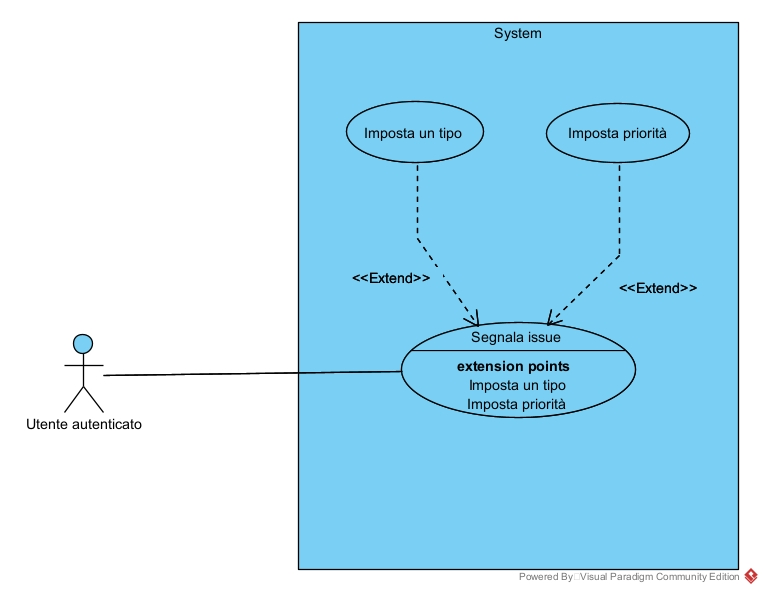
\includegraphics[width=0.8\textwidth]{images/Parziali/BugBoard26_SegnalaIssue.jpg}
    \caption{Use Case2 - \hyperref[sec:RE03]{Requisito funzionale 3.1.3 -  Segnala issue}}
    \label{fig:etichetta}
\end{figure}

\subsubsection{Use Case Diagram parziale 3}\index{Use Case!Assegna issue} \index{Use Case!Visualizza issue assegnate}
\label{sec:UC03}
Il seguente Use Case è un estratto dello Use Case generale. Non aggiunge informazioni al caso d'uso specifico. Serve solamente a focalizzare l'attenzione sul caso/i d'uso specifico/i.
I casi d'uso mostrati sono due: \textit{Segnala issue e Visualizza issue assegnate}. 
\begin{itemize}
    \item \textit{Assegna issue}. L'attore principale è un amministratore. Esso può assegnare una issue a membri del team, ammesso che la issue non risulti già assegnata.
    Il sistema modificherà lo stato della issue da \textit{Todo} a \textit{In Progress} e invierà una notifica all'utente al quale è stata assegata la issue. 
    \item \textit{Visualizza issue assegnate}. L'attore principale è un utente autenticato. Esso può visualizzare l'elenco delle issue che gli sono state assegnate.
\end{itemize} 
\begin{figure}[H]
    \centering
    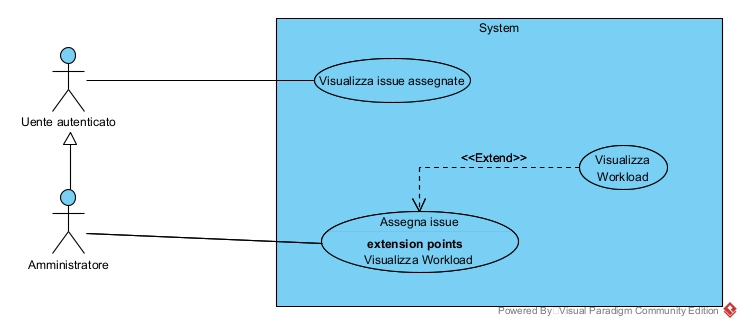
\includegraphics[width=0.8\textwidth]{images/Parziali/BugBoard26_Visualizza&Assegna.jpg}
    \caption{Use Case3 - \hyperref[sec:RE04]{Requisito funzionale 3.1.4 - Assegna issue} e \hyperref[sec:RE07]{Requisito funzionale 3.1.7 - Visualizza issue assegnate}}
    \label{fig:etichetta}
\end{figure}



\subsubsection{Use Case Diagram parziale 4}\index{Use Case!Visualizza riepilogo} \index{Use Case!Visualizza report team}
\label{sec:UC04}
Il seguente Use Case è un estratto dello Use Case generale. Non aggiunge informazioni al caso d'uso specifico. Serve solamente a focalizzare l'attenzione sul caso/i d'uso specifico/i.
I casi d'uso mostrati sono due: \textit{Visualizza riepilogo issue e Visualizza report attività team}. 
\begin{itemize}
    \item \textit{Visualizza riepilogo}. L'attore principale è un utente autenticato. Esso può visualizzare un elenco di tutte le issue e relativi commenti, presenti nel sistema.
    L'elenco è dinamico, nel senso che è possibile ottenere una vista personalizzata delle issue, filtrando, ordinando o ricercando per parametri e perole chiave.
    \item \textit{Visualizza report attività team}. L'attore principale è un amministratore. Esso può visualizzare i report mensili del team, con le metriche e i dettagli per singolo utente. 
\end{itemize}  
Il seguente caso d'uso integra i requisiti funzionali \hyperref[sec:RE08]{RE08}, \hyperref[sec:RE09]{RE09} e \hyperref[sec:RE10]{RE10}, che non
sono rappresentate come casi d'uso autonomi.
\begin{figure}[H]
    \centering
    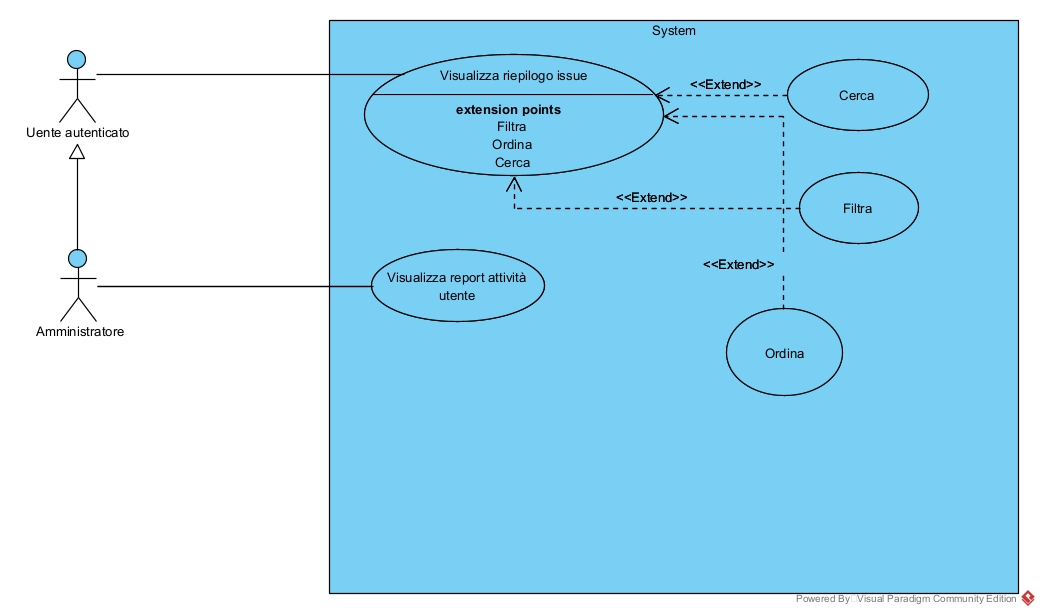
\includegraphics[width=0.8\textwidth]{images/Parziali/BugBoard26_VisualizzaReport&VisualizzaRiepilogo.jpg}
    \caption{Use Case4 - \hyperref[sec:RE05]{Requisito funzionale 3.1.5 -  Visualizza riepilogo issue} e \hyperref[sec:RE06]{ Requisito funzionale 3.1.6 -  Visualizza report team}}
    \label{fig:etichetta}
\end{figure}


\subsubsection{Use Case Diagram parziale 6}\index{Use Case!Visualizza Notifiche}
\label{sec:UC06}
Il seguente Use Case è un estratto dello Use Case generale. Non aggiunge informazioni al caso d'uso specifico. Serve solamente a focalizzare l'attenzione sul caso/i d'uso specifico/i.
In particolare, si pone l'attenzione sulla visualizzazione delle proprie notifiche. 
\begin{figure}[H]
    \centering
    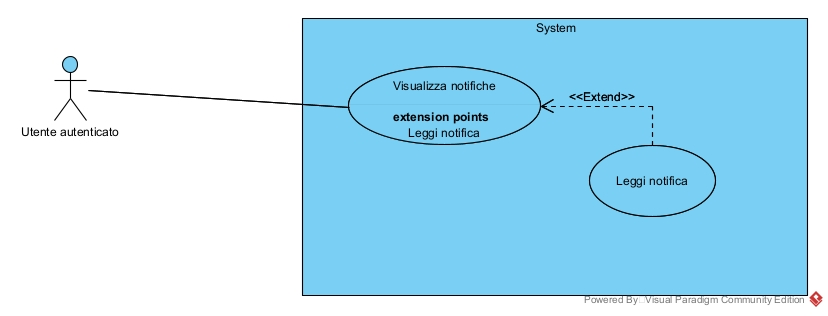
\includegraphics[width=0.8\textwidth]{images/Parziali/visualizzaNotifiche.jpg}
    \caption{Use Case6 - \hyperref[sec:RE11]{Requisito funzionale 3.1.11 - Visualizza Notifiche}}
    \label{fig:etichetta}
\end{figure}

\subsection{Requisiti non funzionali}

Di seguito sono elencati i requisiti non funzionali del sistema \textit{BugBoard26}, classificati secondo le categorie previste dallo standard IEEE Std 830-1998.

\subsubsection{RNF01 - Sicurezza}
Il sistema deve garantire la \textit{segretezza} e l'\textit{integrità} delle informazioni gestite, in quanto critiche per l'azienda. In particolare:
\begin{itemize}
    \item L'accesso alle funzionalità del sistema deve essere consentito esclusivamente ad utenti autenticati, secondo i permessi associati al proprio ruolo (Utente o Amministratore).
    \item Nessuna password deve essere memorizzata all'interno del sistema: la gestione delle credenziali è demandata ad un provider di identità esterno (\textit{Amazon Cognito}).\index{Amazon Web Services (AWS)!Cognito}
    \item La creazione di nuove utenze non può avvenire in autonomia da parte degli utenti, ma richiede necessariamente l'intervento di un Amministratore.
\end{itemize}

\subsubsection{RNF02 - Affidabilità}
Il sistema deve garantire la corretta e costante disponibilità delle proprie funzionalità. Il back-end, distribuito tramite container Docker su infrastruttura Cloud (AWS), è configurato con politiche di riavvio automatico in caso di arresto anomalo, al fine di minimizzare i tempi di interruzione del servizio.\index{Docker}

\subsubsection{RNF03 - Prestazioni}
Il sistema deve garantire tempi di risposta rapidi durante l'interazione con l'utente, in particolare nelle operazioni più frequenti quali la visualizzazione, il filtraggio, l'ordinamento e la ricerca delle issue. La gestione asincrona di alcune operazioni (es. l'invio delle notifiche a seguito dell'assegnazione di una issue, contribuisce a non penalizzare i tempi di risposta percepiti dall'utente durante le richieste principali.

\subsubsection{RNF04 - Usabilità}
L'interfaccia utente deve essere semplice ed intuitiva, tale da consentire l'utilizzo del sistema senza necessità di supporto o di una curva di apprendimento (vedi \hyperref[sec:attori]{Sezione 2.3 - Utenti e attori del sistema}).

\subsubsection{RNF05 - Scalabilità}
L'architettura client-server, organizzata su più livelli \hyperref[sec:analisiArchitettura]{(Sezione 4.1)}, deve consentire l'aggiunta di nuovi client o l'evoluzione del server senza richiedere modifiche sostanziali all'intero sistema.\index{Client-Server}

\subsubsection{RNF06 - Portabilità e indipendenza tra i componenti}
Il front-end e il back-end devono essere componenti indipendenti, comunicanti esclusivamente tramite API REST esposte dal back-end. Deve essere possibile sostituire o modificare il front-end senza alcun impatto sul back-end, e viceversa.

\subsubsection{RNF07 - Manutenibilità}
Il codice del sistema deve essere organizzato secondo un'architettura a livelli e principi di progettazione ad oggetti, al fine di favorire la leggibilità, l'estensibilità e il riutilizzo del codice.

\subsection{Formalizzazione di casi d'uso significativi}
Descrizione tramite tabelle di Cockburn dei casi d'uso significativi.\index{Cockburn}

\subsubsection{Tabella di Cockburn 1}
\label{sec:CKB01}
Tabella di Cockburn del caso d'uso \hyperref[sec:RE03]{Requisito funzionale 3.1.2 - Segnala issue}\index{Issue!Segnalazione}

\begin{longtable}{|p{4cm}|p{12cm}|}
\hline
\textbf{Use Case 2} & \textbf{Segnala Issue} \\ \hline
Goal in Context & Permette agli utenti autenticati di creare una issue con titolo e descrizione e,facoltativamente, 
di inserire un tipo e assegnare un livello di priorità\index{Priorità}  \\ \hline
Preconditions & L'utente ha effettuato l'autenticazione nel sistema \\ \hline
Success End Condition &  L'issue viene registrata nel sistema, risultando visibile con lo stato iniziale di \textit{Todo} \\ \hline
Failed End Condition & L'issue non viene registrata nel sistema e viene visualizzato il messaggio di Errore: \textit{Issue non creata}  \\ \hline
Primary Actor & Utente autenticato  \\ \hline
Trigger & L'utente autenticato sceglie di creare una nuova issue \\ \hline 
Main Scenario & 
\begin{minipage}[t]{\linewidth}
\begin{tabularx}{\linewidth}{p{0.8cm}|X|X}
\textbf{Step} & \textbf{Utente autenticato} & \textbf{Risposta del sistema} \\ \hline
1 & Accede alla sezione \textit{Crea nuova issue} &   \\ \hline
2 & & \hyperref[sec:MU01]{Mostra MU\_1} \\ \hline
3 & Inserisce i campi obbligatori: titolo e descrizione & \\ \hline
4 & Clicca \textit{Crea} &  \\ \hline
5 & & Crea la issue e \hyperref[sec:MU02]{Mostra MU\_2} \\ \hline
6 & Clicca \textit{Ok} & \\ \hline
\end{tabularx}
\end{minipage}

\strut \\ \hline
Extension \textit{\#1} - Imposta una priorità (campo opzionale) &  
\begin{minipage}[t]{\linewidth}
\begin{tabularx}{\linewidth}{p{0.8cm}|X|X}
\textbf{Step} & \textbf{Utente autenticato} & \textbf{Risposta del sistema} \\ \hline
3.a & Sceglie di selezionare una priorità &  \\ \hline
3.a.1 & & Torna allo step 4 del \textit{Main Scenario}
\end{tabularx}
\end{minipage} \strut \\ \hline
Extension \textit{\#2} - Allega un'immagine (campo opzionale)  & 
\begin{minipage}[t]{\linewidth}
\begin{tabularx}{\linewidth}{p{0.8cm}|X|X}
\textbf{Step} & \textbf{Utente autenticato} & \textbf{Risposta del sistema} \\ \hline
3.b & Sceglie di selezionare un tipo &  \\ \hline
3.b.1 & Clicca \textit{Crea} & \\ \hline
3.b.2 & & Torna allo step 4 del \textit{Main Scenario} 
\end{tabularx}
\end{minipage}\strut \\ \hline

Extension \textit{\#3} - Gestione Errore connessione con il Server  & 
\begin{minipage}[t]{\linewidth}
\begin{tabularx}{\linewidth}{p{0.8cm}|X|X}
\textbf{Step} & \textbf{Utente autenticato} & \textbf{Risposta del sistema} \\ \hline
4.c & Clicca su \textit{Crea} &  \\ \hline
4.c.1 & & \hyperref[sec:MU03]{Mostra MU\_3} e torna allo step 3 del \textit{Main Scenario}
\end{tabularx}
\end{minipage}\strut \\ \hline

Extension \textit{\#4} - Campo obbligatorio non specificato  & 
\begin{minipage}[t]{\linewidth}
\begin{tabularx}{\linewidth}{p{0.8cm}|X|X}
\textbf{Step} & \textbf{Utente autenticato} & \textbf{Risposta del sistema} \\ \hline
4.d & Clicca su \textit{Crea} &  \\ \hline
4.d.1 & & \hyperref[sec:MU04]{Mostra MU\_4} e torna allo step 3 del \textit{Main Scenario}
\end{tabularx}
\end{minipage}\strut \\ \hline

Extension \textit{\#5} - L'utente non conferma la creazione  & 
\begin{minipage}[t]{\linewidth}
\begin{tabularx}{\linewidth}{p{0.8cm}|X|X}
\textbf{Step} & \textbf{Utente autenticato} & \textbf{Risposta del sistema} \\ \hline
6.a & Clicca \textit{Annulla} &  \\ \hline
6.a.1 & & Torna allo step 3 del \textit{Main Scenario}
\end{tabularx}
\end{minipage}\strut \\ \hline

\end{longtable}

\subsubsection{Tabella di Cockburn 2} 
\label{sec:CKB02} Tabella di Cockburn del caso d'uso \hyperref[sec:RE04]{Requisito funzionale 3.1.4 - }\index{Issue!Assegna}
 \textit{Assegna Issue} 
\index{Issue!Assegnazione} 
\begin{longtable}{|p{4cm}|p{12cm}|} \hline \textbf{Use Case 3} & \textbf{Assegna Issue} \\ \hline 
Goal in Context & Permette all'amministratore di assegnare una issue ad un utente \\ \hline 
Preconditions & L'amministratore ha effettuato l'accesso al sistema \\ \hline 
Success End Condition & L'issue viene assegnata all'utente prescelto e il suo stato passa a \textit{In Progress} \\ \hline 
Failed End Condition & L'assegnazione non viene completata e viene visualizzato il messaggio di errore: \textit{Impossibile completare l'assegnazione} \\ \hline 
Primary Actor & Amministratore \\ \hline 
Trigger & L'amministratore clicca su \textit{Assegna Issue} \\ \hline 
Main Scenario & \begin{minipage}[t]{\linewidth} 
\begin{tabularx}{\linewidth}{p{0.8cm}|X|X} \textbf{Step} & 
\textbf{Amministratore} & \textbf{Risposta del sistema} \\ \hline 
1 & Accede alla sezione \textit{Assegna Issue} & \\ \hline 
2 & & \hyperref[sec:MU05]{Mostra MU\_1} \\ \hline 
3 & Seleziona la issue da assegnare e seleziona l'utente & \\ \hline 
4 & Clicca \textit{Assegna} & \\ \hline 
5 & & Mostra \hyperref[sec:MU06]{MU\_2} \\ \hline 
6 & Clicca \textit{OK} & \\ \hline 
\end{tabularx} 
\end{minipage} \strut \\ \hline 

Extension \textit{\#1} - Utente e/o Issue non selezionati & \begin{minipage}[t]{\linewidth} 
\begin{tabularx}{\linewidth}{p{0.8cm}|X|X} \textbf{Step} & \textbf{Amministratore} & \textbf{Risposta del sistema} \\ \hline 
4.a & Non seleziona l'utente e/o la issue & \\ \hline 
4.a.1 & Clicca su \textit{Assegna} & \\ \hline 
4.a.2 & & \hyperref[sec:MU07]{Mostra MU\_3} e torna allo step 3 del \textit{Main Scenario} 
\end{tabularx} 
\end{minipage} \strut \\ \hline 

Extension \textit{\#2} - Errore di rete & \begin{minipage}[t]{\linewidth} \begin{tabularx}{\linewidth}{p{0.8cm}|X|X} \textbf{Step} & \textbf{Amministratore} & \textbf{Risposta del sistema} \\ \hline 
4.b & Clicca su \textit{Assegna} & \\ \hline 
4.b.1 & & \hyperref[sec:MU08]{Mostra MU\_4} \\ \hline 
4.b.2 & Clicca \textit{OK} & \\ \hline 
4.b.3 & & Torna allo step 3 del \textit{Main Scenario} 
\end{tabularx} 
\end{minipage} \strut \\ \hline 
\end{longtable}

\subsection{Prototipazione visuale del caso d'uso 3.3.3 Segnala Issue}
\index{Mockup}
Le seguenti figure rappresentano la prototipazione visuale via Mock-up delle relative interfacce utente. Non sono da intendersi come rappresentativi dell'aspetto finele 
della schermata, ma solamente un mezzo per comunicare l'idea dell'interfaccia grafica del prodotto software.

\subsubsection{Segnala Issue - Mockup 1}
\label{sec:MU01}
\begin{figure}[H]
    \centering
    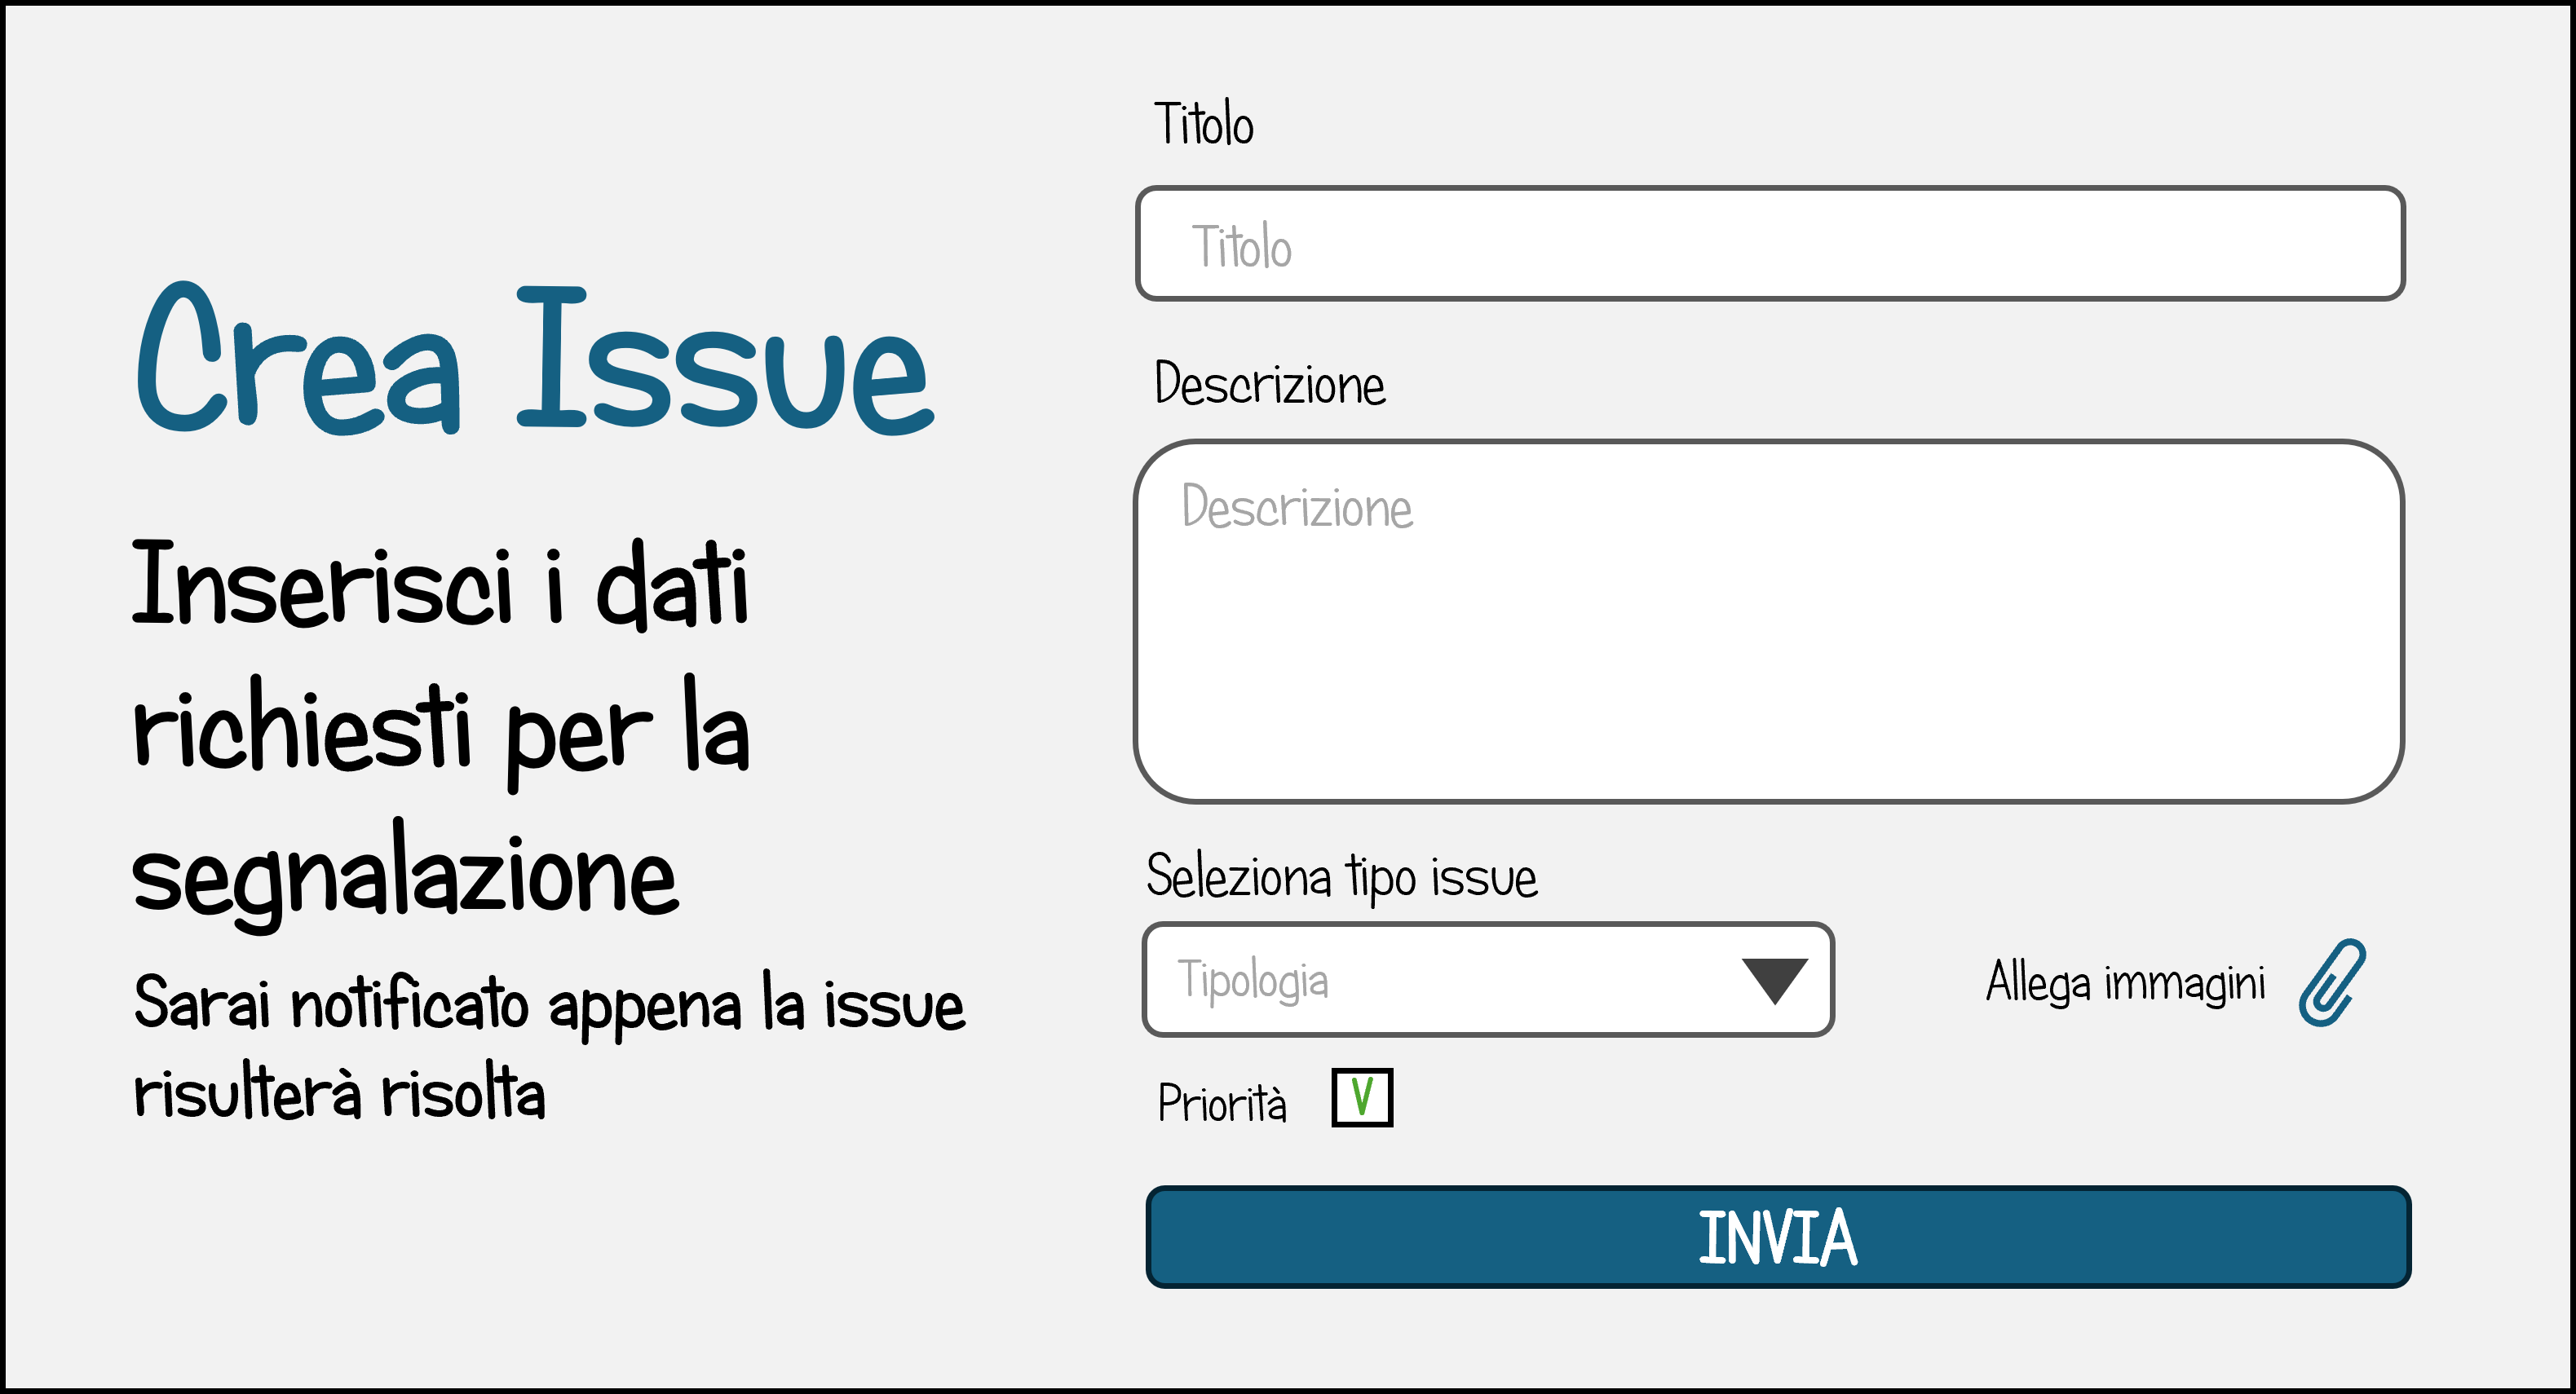
\includegraphics[width=1.0\textwidth]{images/SegnalaIssueMockup/MU_1.png}
    \caption{Mockup 1 - Crea issue riferito a \hyperref[sec:CKB01]{3.4.1 Tabella di Cockburn 1 - Step 2 del Main Scenario}}
    \label{fig:MU01}
\end{figure}

\subsubsection{Segnala Issue - Mockup 2}
\label{sec:MU02}
\begin{figure}[H]
    \centering
    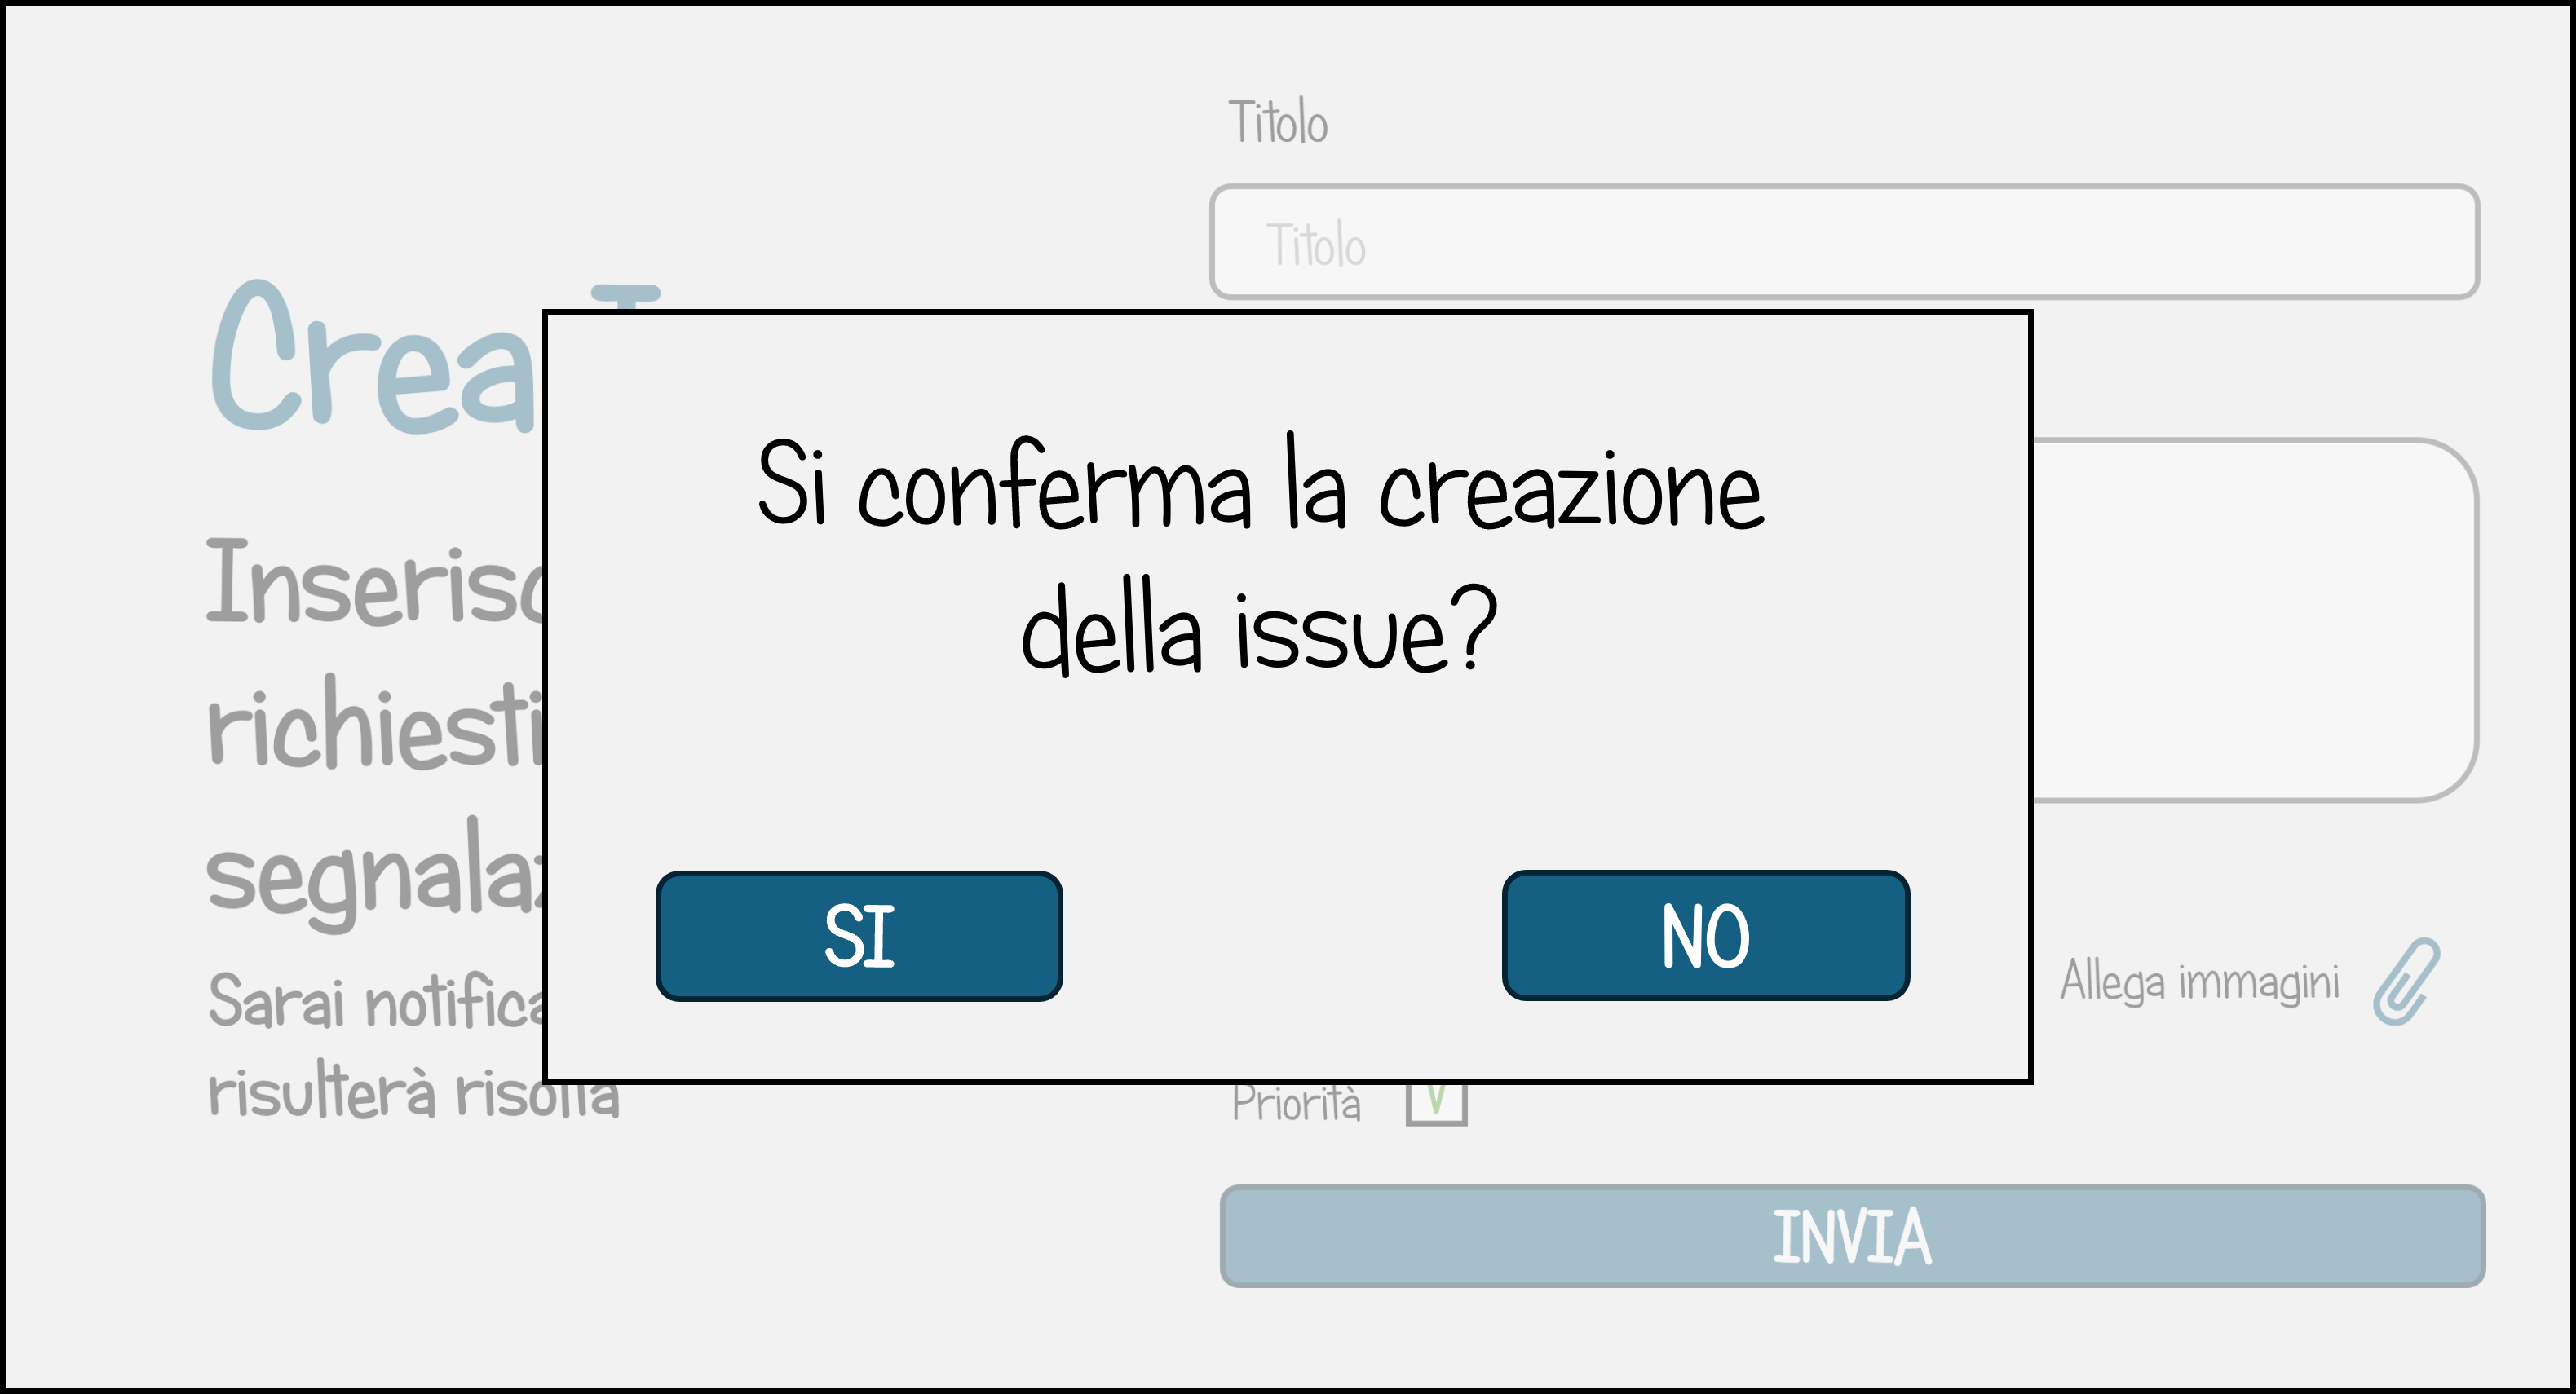
\includegraphics[width=1.0\textwidth]{images/SegnalaIssueMockup/MU_2.png}
    \caption{Mockup 2 - Crea issue riferito a \hyperref[sec:CKB01]{3.4.1 Tabella di Cockburn 1 - Step 5}}
    \label{fig:MU02}
\end{figure}

\subsubsection{Segnala Issue - Mockup 3}
\label{sec:MU03}
\begin{figure}[H]
    \centering
    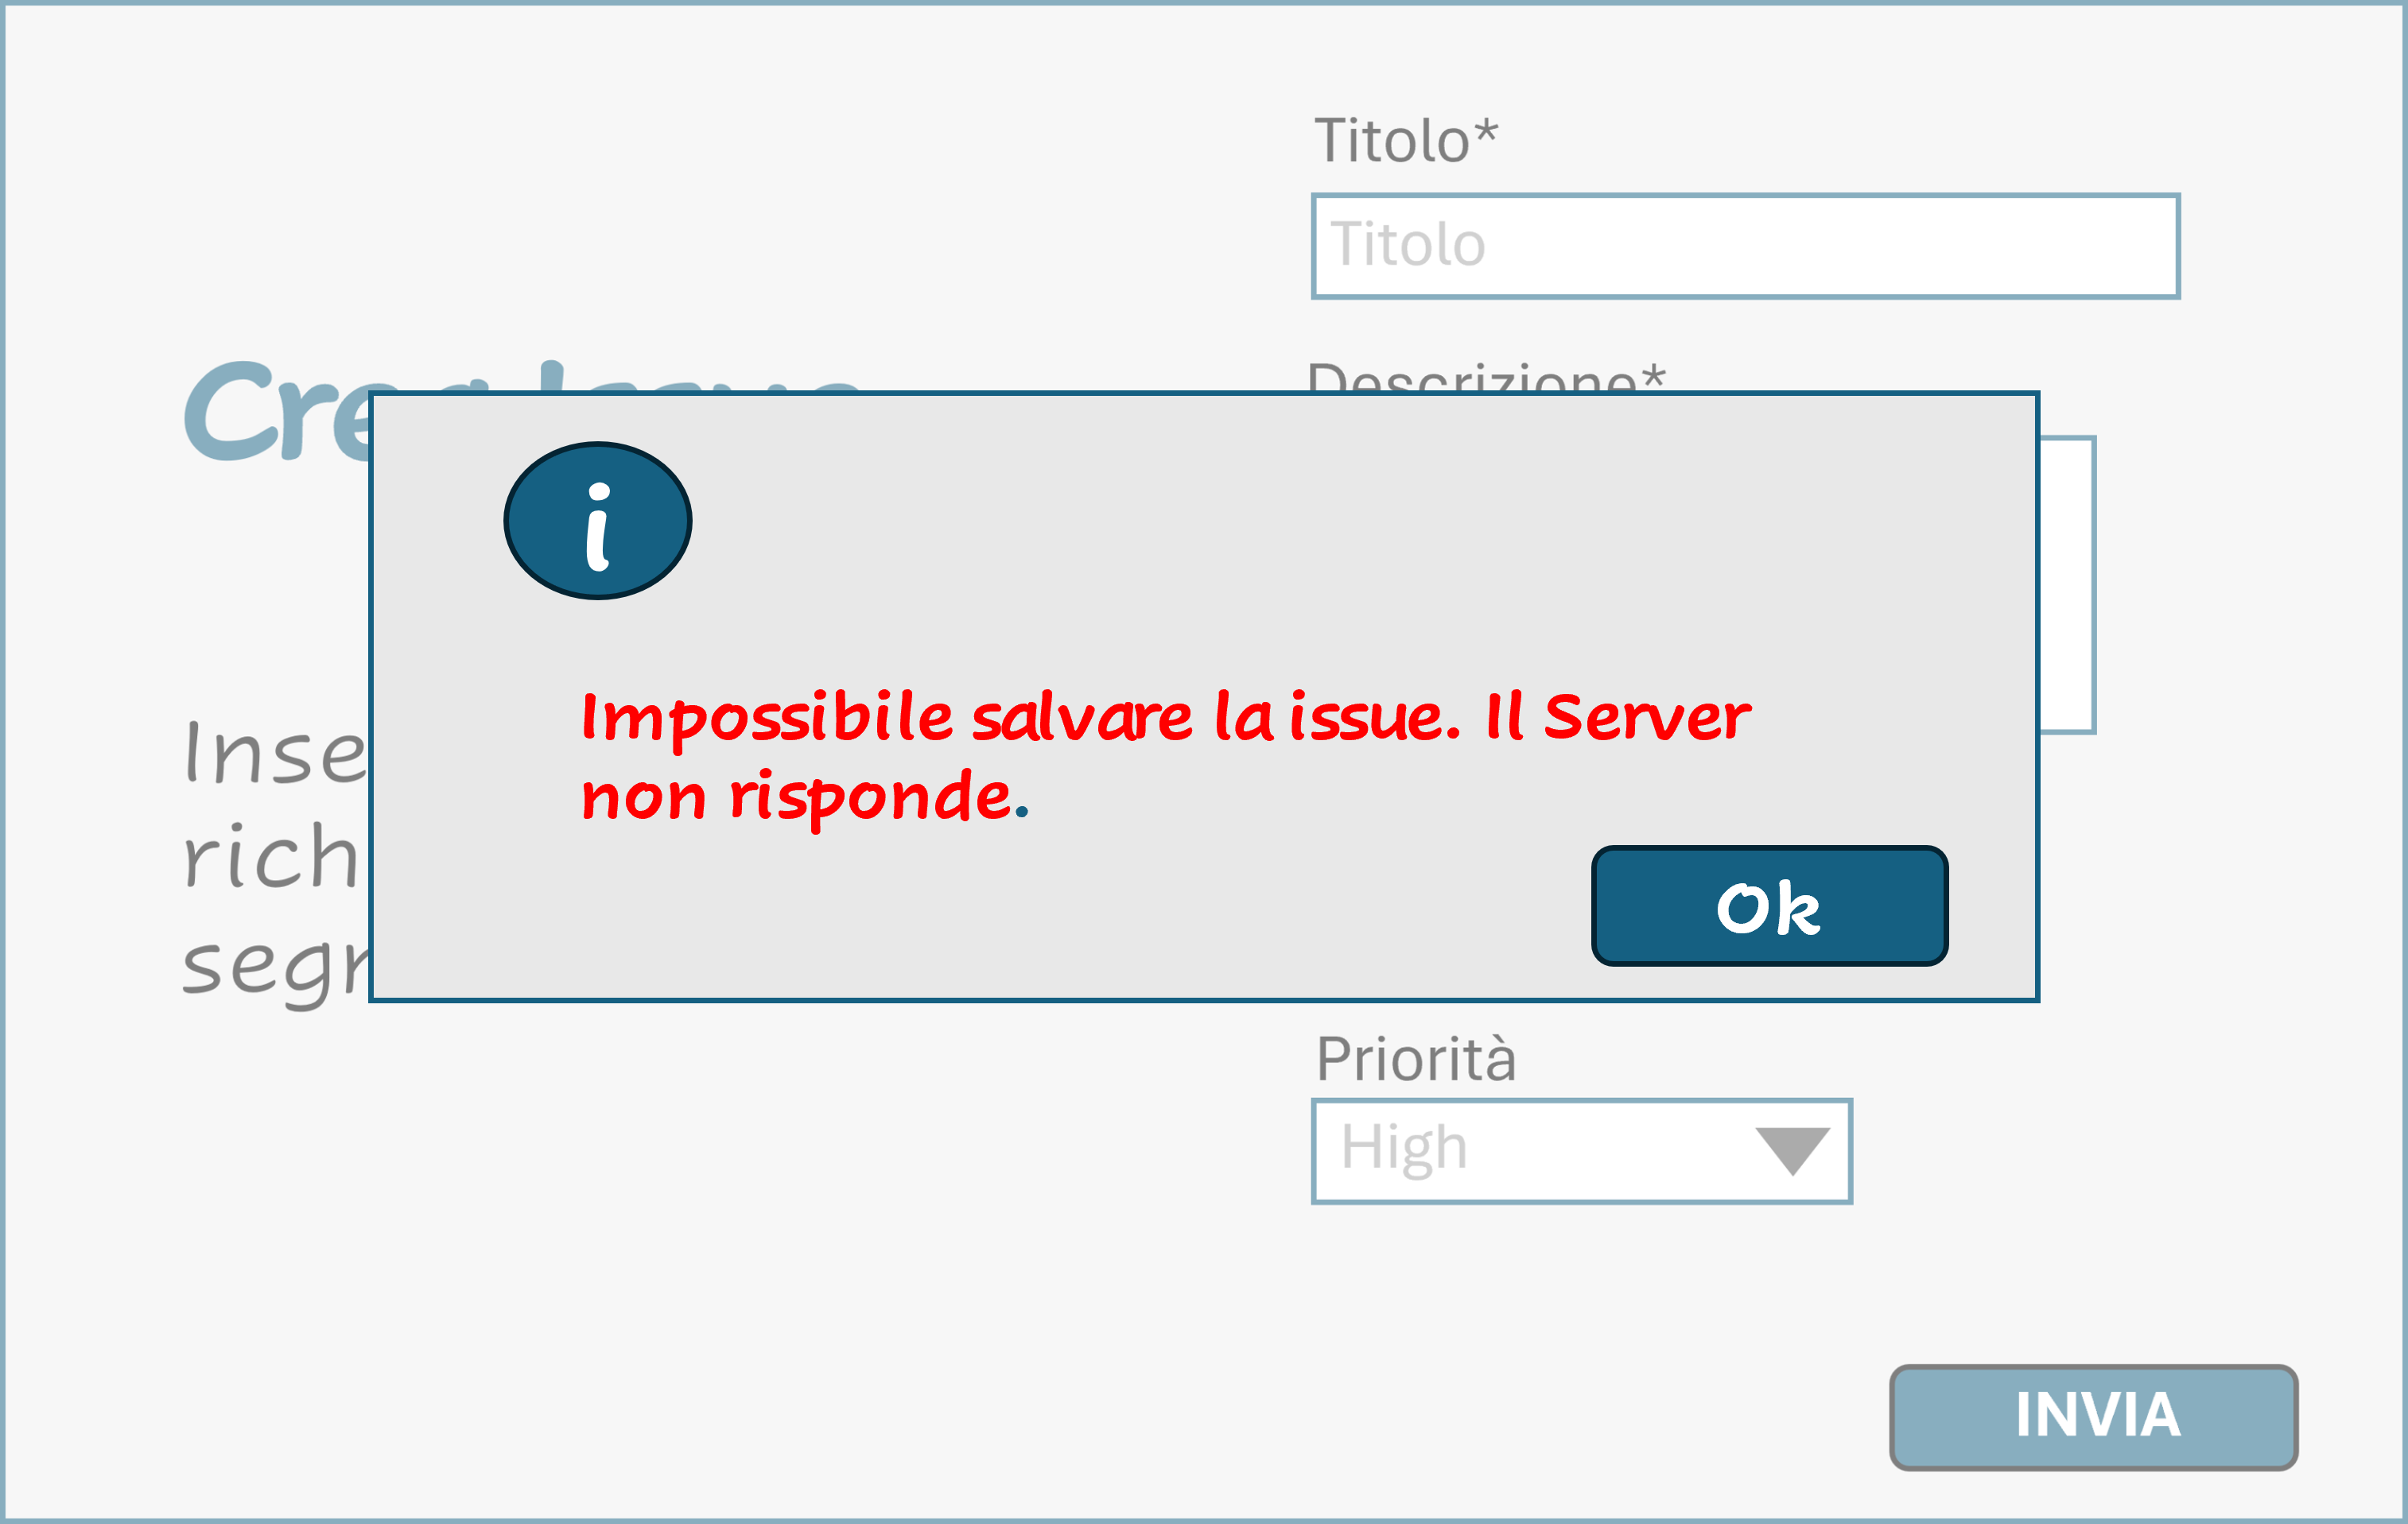
\includegraphics[width=1.0\textwidth]{images/SegnalaIssueMockup/MU_3.png}
    \caption{Mockup 3 - Crea issue riferito a \hyperref[sec:CKB01]{3.4.1 Tabella di Cockburn 1 - Step 4.c.1}}
    \label{fig:MU03}
\end{figure}

\subsubsection{Segnala Issue - Mockup 4}
\label{sec:MU04}
\begin{figure}[H]
    \centering
    
\includegraphics[width=1.0\textwidth]{images/SegnalaIssueMockup/MU_4.png}
    \caption{Mockup 4 - Crea issue riferito a \hyperref[sec:CKB01]{3.4.1 Tabella di Cockburn 1 - Step 4.b.1}}
    \label{fig:MU04}
\end{figure}

\subsection{Prototipazione visuale del caso d'uso Assegna Issue} 
\index{Mockup} 
Le seguenti figure rappresentano la prototipazione visuale via Mock-up delle relative interfacce utente. Non sono da intendersi come rappresentativi dell'aspetto finale della schermata, ma solamente un mezzo per comunicare l'idea dell'interfaccia grafica del prodotto software. 

\subsubsection{Assegna Issue - Mockup 1} 
\label{sec:MU05} 
\begin{figure}[H] \centering 
\includegraphics[width=1.0\textwidth]{images/AssegnaIssueMockup/MU_1.png} 
\caption{Mockup 1 - Assegna issue riferito a \hyperref[sec:CKB02]{Tabella di Cockburn 2 - Step 2 del Main Scenario}} 
\label{fig:MU05} 
\end{figure} 

\subsubsection{Assegna Issue - Mockup 2} 
\label{sec:MU06} 
\begin{figure}[H] \centering 
\includegraphics[width=1.0\textwidth]{images/AssegnaIssueMockup/MU_2.png} 
\caption{Mockup 2 - Assegna issue riferito a \hyperref[sec:CKB02]{Tabella di Cockburn 2 - Step 5 del Main Scenario}} 
\label{fig:MU06} 
\end{figure} 

\subsubsection{Assegna Issue - Mockup 3} 
\label{sec:MU07} 
\begin{figure}[H] \centering 
\includegraphics[width=1.0\textwidth]{images/AssegnaIssueMockup/MU_3.png} 
\caption{Mockup 3 - Assegna issue riferito a \hyperref[sec:CKB02]{Tabella di Cockburn 2 - Step 4.a.2}} 
\label{fig:MU07} 
\end{figure} 

\subsubsection{Assegna Issue - Mockup 4} 
\label{sec:MU08} 
\begin{figure}[H] \centering 
\includegraphics[width=1.0\textwidth]{images/AssegnaIssueMockup/MU_4.png} 
\caption{Mockup 4 - Assegna issue riferito a \hyperref[sec:CKB02]{Tabella di Cockburn 2 - Step 4.b.1}} 
\label{fig:MU08} 
\end{figure}

\newpage
\section{Documento di design del sistema}
\label{sec:analisiArchitettura}
\subsection{Analisi dell'Architettura}
Il progetto BugBoard26 è stato sviluppato con un'architettura \textit{\textbf{client-server}} (fig. 1) organizzata su tre livelli che comunicano tramite API REST. Tale organizzazione è suddivisa in: \index{Client-Server}
\begin{itemize}
    \item Presentation Layer (Client)
    \item Bussines Logic Layer (Server)
    \item Data Layer (Persistenza)
\end{itemize}

Questa scelta consente di ottenere numerosi vantaggi pratici. Tra i principali si evidenzia la centralizzazione dei dati: le informazioni vengono gestite dal server e distribuite ai client che ne fanno richiesta, garantendo così maggiore controllo e coerenza. Un ulteriore beneficio riguarda la sicurezza, in particolare per quanto concerne la gestione dell’autenticazione degli utenti, che è affidata al server e risulta quindi più efficace e affidabile.
Un altro aspetto particolarmente rilevante è la scalabilità: il modello permette infatti di aggiungere nuovi client o server senza apportare modifiche sostanziali all’intero sistema.
Per tutti questi motivi, la decisione di utilizzare il modello Client-Server rappresenta
la soluzione più coerente per lo sviluppo del software. 
\begin{figure}[H]
    \centering
    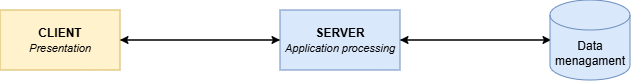
\includegraphics[width=1.0\textwidth]{images/Architettura/Client-Server.png}
    \caption{Schema architetturale 1 - Architettura Client-Server}
    \label{fig:etichetta}
\end{figure}


\subsubsection{Server}
Il sistema adotta un’architettura basata sul \textbf{pattern MVC} (Model-View-Controller), estesa attraverso l’introduzione di ulteriori livelli applicativi, come Service, DTO, Mapper e moduli di autenticazione. Questa organizzazione consente una separazione ancora più marcata delle responsabilità: i \textbf{Controller} si occupano della gestione delle richieste HTTP, i \textbf{Services} della logica di business, i \textbf{DTO} e \textbf{Mapper} facilitano lo scambio e la trasformazione dei dati, la componente \textbf{View} è rappresentata dal processo di serializzazione (da Object a JSON) e deserializzazione (da JSON a Object) dei dati trasferiti dal o verso il client, mentre la componente \textbf{Repositories} rappresenta l'interfaccia che fornisce i servizi per la comunicazione con il sistema di persistenza dei dati. \index{DTO} \index{MVC}

L'architettura appena illustrata è rappresentata dal seguente Component Diagram UML.
\begin{figure}[H]
    \centering
    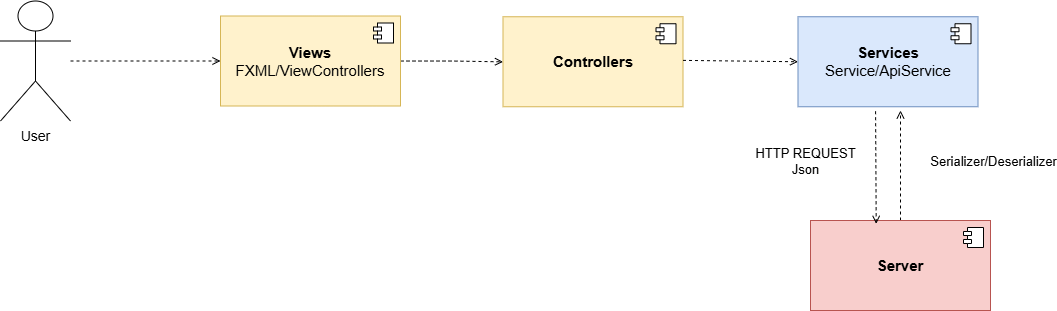
\includegraphics[width=1.0\textwidth]{images/Architettura/ComponentDiagramClient.png}
    \caption{Schema architetturale 2 - Component Diagram del backend}
    \label{fig:etichetta}
\end{figure}


\subsubsection{Persistenza}
La persistenza fisica dei dati è sviluppata mediante l'utilizzo di un DBMS relazionale disaccoppiato dal resto del sistema tramite l'interfaccia Repository.
Il database relazionale garantisce la persistenza dei dati in modo sicuro. L'interazione con esso avviene tramite il livello \textbf{Repositories}, che incapsula le operazioni di accesso ai dati, mantenendo separata la logica applicativa dalla persistenza dei dati.
\index{Database}
\subsubsection{Client}
L'architettura del \textit{frontend} è basata sul pattern architetturale MVC (\textit{Model-View-Controller}) esteso con moduli ausiliari per una corretta separazione delle responsabilità. In particolare, il modulo ViewController, insieme alle risorse FXML, costituiscono il livello di presentazione. I ViewController gestiscono le pagine FXML garantendo il corretto funzionamento della GUI. Il modulo Service si occupa della logica di business, riducendo le responsabilità dei Controller, che ricevono gli eventi generati dalla View, richiamano i servizi che comunicano con il back-end tramite le API REST esposte, e aggiornano il Model con i dati ricevuti.
L'architettura appena illustrata è rappresentata dal seguente Component Diagram UML.\index{MVC}
\begin{figure}[H]
    \centering
    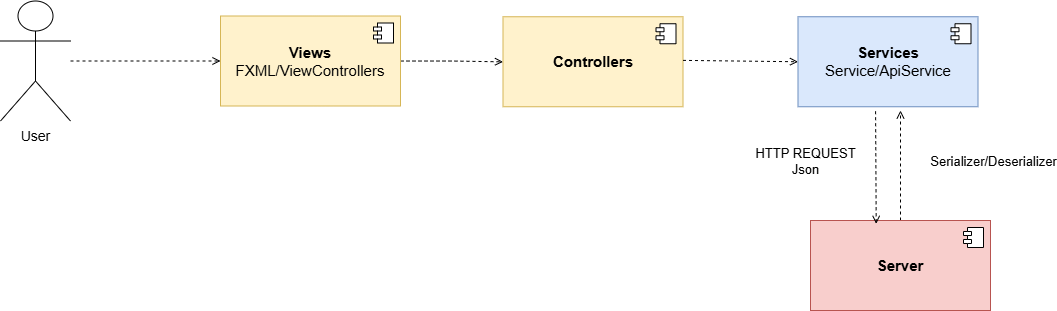
\includegraphics[width=1.0\textwidth]{images/Architettura/ComponentDiagramClient.png}
    \caption{Schema architetturale 3 - Component Diagram del frontend}
    \label{fig:etichetta}
\end{figure}


\subsection{Scelte tecnologiche e motivazioni}
La scelta tecnologica più rilevante, riferita all'intero sistema, riguarda la gestione dell'autenticazione. L'autenticazione è stata gestita interamente tramite \textbf{Amazon Cognito}, configurato su un server nella regione di Milano. Tramite un'apposita pagina UI del frontend, l'utente può richiedere di effettuare il login: la richiesta lo indirizza verso la \textit{Hosting UI} di Cognito, una pagina di autenticazione esterna al sistema \textit{BugBoard26}. Contestualmente, il frontend apre un server temporaneo in ascolto sulla porta 9090, in attesa della risposta (positiva o negativa) da parte di Cognito.\index{Amazon Web Services (AWS)!Cognito}

Come indicato nel documento dei requisiti, il sistema non permette la registrazione spontanea a BugBoard26: la creazione di una nuova utenza richiede necessariamente l'intervento di un Amministratore. La registrazione di una nuova utenza (sia essa di ruolo Admin che User) avviene interamente all'interno di BugBoard26: il frontend acquisisce email e ruolo del nuovo utente, mentre il backend, oltre a persistere i dati nel database, invia una richiesta API a Cognito per aggiungere l'utente al pool di utenti già esistente. Cognito provvede quindi all'invio di un'email al nuovo utente contenente una password temporanea, forzando il cambio della password al primo accesso.\index{Database}

Questa scelta garantisce un sistema di autenticazione semplice e, soprattutto, sicuro, poiché \textbf{nessuna password viene memorizzata all'interno del sistema}.


Nei paragrafi successivi vengono presentate le principali scelte tecnologiche adottate nel sistema, suddivise per \textit{Client}, \textit{Persistenza} e \textit{Server}.



\subsubsection{Server} 
Per lo sviluppo del \textbf{backend} abbiamo utilizzato Spring Boot (v. 3.2.2), un framework Java che facilita la creazione di API REST grazie al supportos per la gestione di richieste HTTP e l'integrazioni di componenti Spring come Spring MVC. Grazie all'integrazione di Spring Data JPA (Jakarta Persistence API) e Hibernate, i Repositories si occupano delle operazione di lettura e scrittura dei dati (CRUD), delegando al sistema di persistenza la sola gestione fisica delle informazioni.
Tale approccio migliora la manutenibilità, la scalabilità e la chiarezza del codice. \index{MVC} \index{Spring Boot}

Il Server è stato pensato e predisposto per essere containerizzato (con Docker) e messo in opera utilizzando servizi di Cloud Computing (Amazon Web Services). \index{Docker}


\subsubsection{Persistenza} Per la persistenza dei dati è stato scelto PostgreSQL, un DBMS relazionale open-source, affidabile e altamente stabile. Questa scelta è coerente con la natura fortemente relazionale del dominio: le entità principali (Users, Issues, Notifications) sono legate da relazioni ben definite con vincoli di integrità referenziale (es. una Issue ha sempre un reporter e opzionalmente un assegnatario) PostgreSQL è stato scelto per diversi fattori. Inoltre, PostgreSQL si integra facilmente con il
framework Spring Boot e tecnologie JPA/Hibernate. \index{PostgreSQL} \index{Spring Boot}

\subsubsection{Client} Per lo sviluppo del front-end è stato scelto JavaFX, un framework per la realizzazione di applicazioni desktop in Java. Tale scelta è stata motivata da diversi fattori. Tra i principali motivi, essendo il \textit{backend} sviluppato in Java, l'utilizzo di JavaFX permette di avere \textbf{coerenza tecnologica} e di riutilizzare competenze e strumenti su entrambe le componenti del sistema. Altra motivazione decisiva è il supporto nativo di JavaFX con il pattern \textit{MVC}, che favorisce naturalmente la separazione tra interfaccia grafica e logica di presentazione, tramite il formato FXML. Inoltre, rispetto ad alternative come Swing, JavaFX offre un supporto più moderno per componenti grafici, tramite CSS, e gestione di layout responsive, mantentendo  la stessa capacità di comunicare con il back-end esclusivamente tramite chiamate HTTP verso le API REST esposte, senza alcuna dipendenza diretta dal codice del server.\index{JavaFX / FXML}

\newpage
\section{Documento di Design del Software}


\subsection{Descrizione dello schema di persistenza dei dati}
Nella Figura 15 viene mostrato il diagramma UML del database. \index{Database}
\begin{figure}[H]
    \centering
    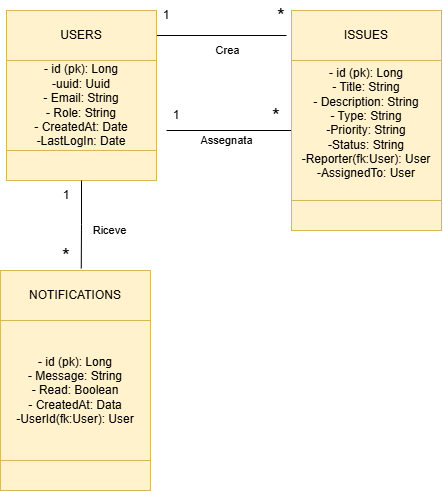
\includegraphics[width=0.7\textwidth]{images/Architettura/Database.png}
    \caption{Schema architetturale 3 - Diagramma UML Database}
    \label{fig:etichetta}
\end{figure}


\index{Class Diagram}
\subsection{Class Diagram di Design} Di seguito sono riportati i class diagram del Server. Si è deciso di dividere il class diagram in vari diagrammi separati, organizzati per funzionalità, per semplificare la consultazione del documento. Inoltre, abbiamo riportato tutte le classi Model in un unico diagramma dettagliato, ogni volta che saranno coinvolte in associazioni nelle varie funzionalità le classi saranno rappresentate in forma ridotta.
\subsubsection{Class Diagram 1- Model}Il seguente class diagram rappresenta per esteso e in modo dettagliato le classi del Model. In seguito verranno riportate solo in forma ridotta.
\begin{figure}[H]
    \centering
    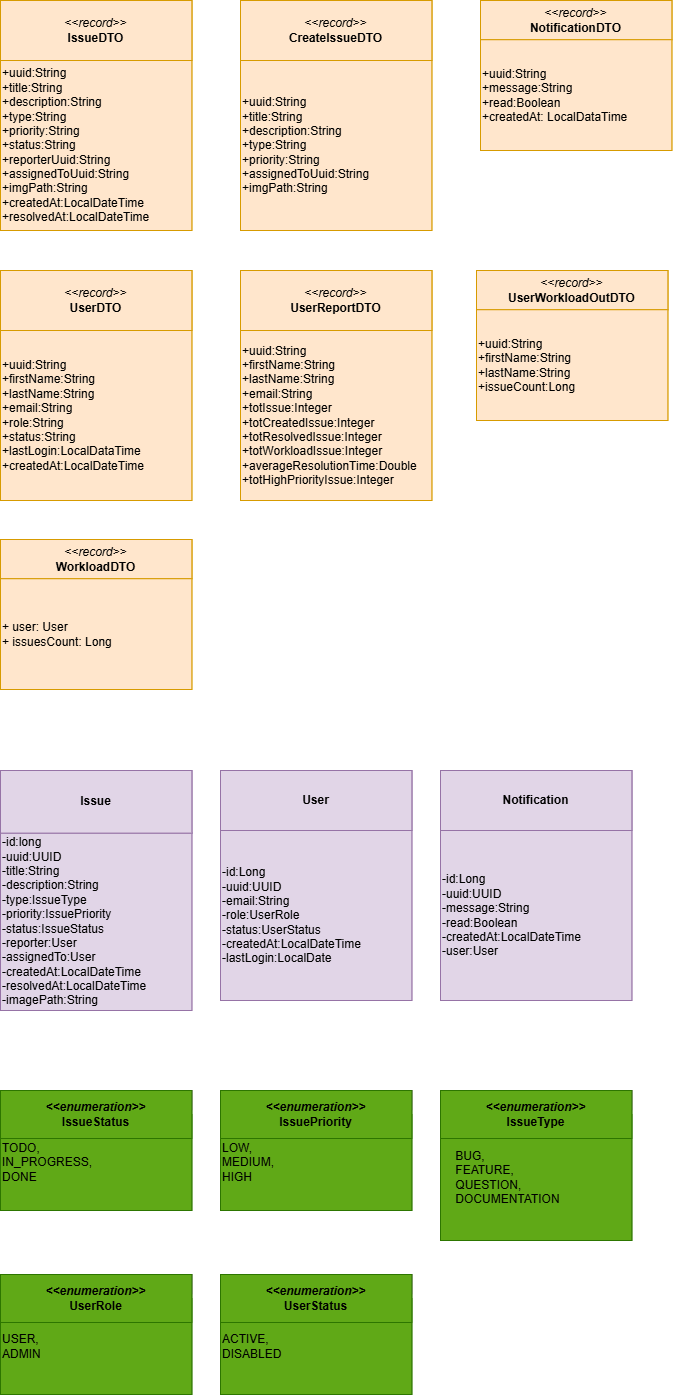
\includegraphics[width=0.7\textwidth]{images/BackendCD/Model.png}
    \caption{Class Diagram 1 - Model dettagliato}
    \label{fig:ClassDiagramModel}
\end{figure}



\subsubsection{Class Diagram 2- Funzionalità 2}Il seguente class diagram rappresenta le classi coninvolte nella funzioanlità 2
\begin{figure}[H]
    \centering
    
\includegraphics[width=1.0\textwidth]{images/BackendCD/Funzionalità 2.png}
    \caption{Class Diagram 2 - Funzionalità 2}
    \label{fig:ClassDiagramFunz2}
\end{figure}

\subsubsection{Class Diagram 3- Funzionalità 3}Il seguente class diagram rappresenta le classi coninvolte nella funzioanlità 3
\begin{figure}[H]
    \centering
    
\includegraphics[width=1.0\textwidth]{images/BackendCD/Funzionalità 3.png}
    \caption{Class Diagram 3 - Funzionalità 3}
    \label{fig:ClassDiagramFunz3}
\end{figure}

\subsubsection{Class Diagram 4- Funzionalità 4 e 14}Il seguente class diagram rappresenta le classi coninvolte nelle funzioanlità 4 e 14
\begin{figure}[H]
    \centering
    
\includegraphics[width=1.0\textwidth]{images/BackendCD/Funzionalità 4 e 14.png}
    \caption{Class Diagram 4 - Funzionalità 4 e 14}
    \label{fig:ClassDiagramFunz4e14}
\end{figure}


\subsubsection{Class Diagram 5- Funzionalità 11}Il seguente class diagram rappresenta le classi coninvolte nella funzioanlità 11
\begin{figure}[H]
    \centering
    
\includegraphics[width=1.0\textwidth]{images/BackendCD/Funzionalità 11.png}
    \caption{Class Diagram 5 - Funzionalità 11}
    \label{fig:ClassDiagramFunz11}
\end{figure}

\subsubsection{Class Diagram 6- Funzionalità 17}Il seguente class diagram rappresenta le classi coninvolte nella funzioanlità 17
\begin{figure}[H]
    \centering
    
\includegraphics[width=1.0\textwidth]{images/BackendCD/Funzionalità 17.png}
    \caption{Class Diagram 6 - Funzionalità 17}
    \label{fig:ClassDiagramFunz17}
\end{figure}

\subsection{Package Diagram Frontend}
\begin{figure}[H]
    \centering
    
\includegraphics[width=1.0\textwidth]{images/Architettura/Frontend - Package Diagram.png}
    \caption{Package Diagram - Frontend}
    \label{fig:PackageDiagram - Frontend}
\end{figure}

\subsection{Descrizione e motivazione delle scelte di software design adottate} Di seguito una lista dei principali design pattern utilizzati nel sistema \textit{BugBoard26}. 
\begin{itemize}
    \item \textbf{Dependency injection:} La DI è stata molto utilizzata nello sviluppo del sistema (sia lato Client che lato Server). Questa scelta comporta diversi vantaggi. \index{Dependency Injection}
    \textbf{Basso accoppiamento:} le classi dipendono da astrazioni (interfacce come \texttt{IssueService}, \texttt{IssueRepository}) e non da implementazioni concrete, coerentemente con il principio di Dependency Inversion (SOLID). Questo permette di sostituire un'implementazione (es. \texttt{IssueServiceImpl}) senza modificare le classi che la utilizzano. \index{Principi SOLID}
    \textbf{Testabilità:} la possibilità di iniettare mock delle interfacce al posto delle implementazioni reali ha semplificato la scrittura di test di unità (es. testare IssueServiceImpl iniettando il mock \texttt{IssueRepository}, senza necessità di un database reale). \index{Database}
    \textbf{Been di Spring} il ciclo di vita e la creazione delle istanze (bean) sono gestiti da Spring, evitando la duplicazione di logica di istanziazione sparsa nel codice.
    \item \textbf{Singleton:} Il pattern Singleton viene utilizzato per la classe \texttt{AuthSession} del \textit{frontend}. Crea una istanza della classe alla quale è possibile accedere dall'esterno per ottenere il tocken necessario per costruire una corretta chiamata API al \textit{backend}. Naturalmente espone un costruttore privato per evitare la creazione di ulteriori istanze della classe. \index{Singleton}
    \item \textbf{Event-Listener}: L'\textit{Event-Listener} è un pattern architetturale peculiare di Spring. È stato scelto in sostituzione del design pattern Observer, di cui è una specializzazione in chiave tecnologica Spring. Si occupa della gestione degli eventi, disaccoppiando il componente che genera un evento (\textit{publisher}) da quello che deve gestire le conseguenze (\textit{listener}), senza che il primo debba conoscere direttamente il secondo.\index{Event-Listener / Observer}

    Nel sistema, questo meccanismo è utilizzato per la gestione delle notifiche. Quando un amministratore assegna una \textit{Issue} ad un utente, l'\texttt{IssueService} non invoca direttamente il servizio di notifica, ma pubblica un evento (es. \texttt{IssueAssignedEvent}) tramite \texttt{ApplicationEventPublisher}, contenente i riferimenti necessari (identificativo della issue e dell'utente assegnatario). Un componente listener dedicato (es. \texttt{NotificationEventListener}), registrato tramite l'annotazione \texttt{@EventListener}, intercetta l'evento e si occupa di creare la relativa notifica nel model e nel database. \index{Database}Questa scelta comporta due importanti vantaggi. In primo luogo genera un \textbf{basso accoppiamento}. L'\texttt{IssueService} non ha alcuna dipendenza diretta dal servizio di notifica, rispettando il principio SOLID di \textit{Single Responsibility}: la logica di assegnazione della issue resta separata dalla logica di generazione delle notifiche. Inoltre, è possibile aggiungere ulteriori listener per lo stesso evento senza modificare il codice del componente publisher.\index{Principi SOLID}
\end{itemize}

Oltre ai Pattern appena mostrati, nel sistema \textit{Bugboard26} sono state prese alcune scelte di Design per rispettare i principi SOLID e per ottenere un \textbf{basso accoppiamento e un'alta coesione}.Tra le principali spiccano l'utilizzo di classi \textbf{DTO} (\texttt{Data Transfer Object}) utilizzati per disaccoppiare il Model dallo strato di trasferimento dei dati (la View del backend è il serializzatore/deserializzatore di Spring). Inoltre, è usato per mascherare i Model mostrando al richiedente solamente i dati a cui ha effettivamente accesso. Le classi \textbf{Mapper} si occupano della conversione tra i Model e i DTO.\index{DTO}

Le classi \texttt{Services} sono organizzate secondo una gerarchia che parte dall'interfaccia Service. Essa ci permette di mantenere il disaccoppiamento tra i \textit{Controller} e le classi \textit{Service} concrete. Oltre a questa gerarchia, si è progettata una struttra divisa per tipologia di richiesta ai \texttt{Repositories}: lettura (\textit{read}) e scrittura (\textit{write}). Questa distinzione netta permette un'alta manutenibilità del codice data la semplicità nella localizzazione di eventuali errori. 

La classe \texttt{IssueSpecification} svolge un ruolo cruciale per la manutenibilità e la scalabilità del codice. Introducendo questo componente, è stato possibile evitare una complessa struttura di \textit{if-else} nidificati per la gestione dei filtri di ricerca, delegando la logica di filtraggio delle issue a un'architettura più snella e facilmente estendibile.

Nel \textit{frontend} non è possibile utilizzare una semplice Dependency Injection perchè i \texttt{ViewController} di JavaFX non hanno costruttore. Il primo metodo eseguito è il metodo \texttt{initialize()}, quindi si è deciso di usare un nuovo metodo \texttt{initDependency()} chiamato dal \texttt{DashboardViewController} in cui si settano le dipendenze esterne (Controller e Service), esso verrà eseguito subito dopo l'esecuzione del \texttt{initialize()} (nel quale ci sono solamente creazione di componenti grafici, ma non il caricamento dei dati al loro interno). \index{Dependency Injection} \index{JavaFX / FXML}

Per avere un basso accoppiamento e un'alta coesione nelle classi \texttt{ViewController} del \textit{frontend} si è spostata la logica di presenzazione grafica ad alcune classi di supporto, alle quali i \texttt{ViewController} delegano la creazione di tabelle, grafici, badge, ect. Tutti gli stili grafici sono raggruppati in una classe CSS \texttt{style.css}. 
 

\subsection{Strumento di Versioning} Abbiamo adottato un approccio di versioning basato su \textbf{Github}. Per la gestione del versionamento del codice sorgente e della documentazione è stato utilizzato GitHub. È stato adottato un unico repository per l'intero progetto, organizzato nelle seguenti directory principali:\index{GitHub}
\begin{itemize}
    \item \texttt{Backend/}: codice sorgente del server Spring Boot. \index{Spring Boot}
    \item \texttt{Frontend/}: codice sorgente del client JavaFX.\index{JavaFX / FXML}
    \item \texttt{Documentazione/}: documentazione di progetto (SRS, mockup, diagrammi).
\end{itemize}

Il repository è raggiungibile al seguente link: \url{https://github.com/ManuelMontuori/BugBoard26}

Il report delle attività del team sono presentate in questa schermata estratta da GitHub. 
\begin{figure}[H]
    \centering
    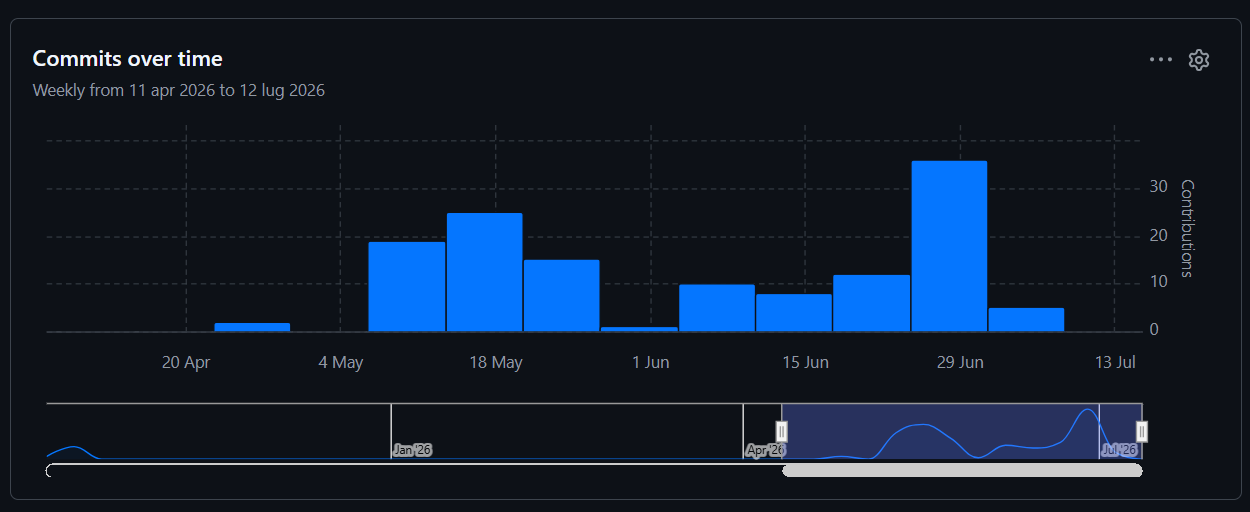
\includegraphics[width=1.0\textwidth]{images/Github.png}
    \caption{Report Github}
    \label{fig:githubReport}
\end{figure}

\subsection{Containerizzazione, build automatica e Cloud Deploy} Il \textbf{backend} è stato containerizzato utilizzando \textit{Docker} e caricato su una macchina virtuale AWS (\textit{Amazon Web Services}). \index{Amazon Web Services (AWS)} \index{Docker}


\subsubsection{Build automatica}

La build del back-end è automatizzata tramite \textbf{Maven} (file \texttt{pom.xml}), che gestisce la risoluzione delle dipendenze del progetto e la generazione dell'artefatto JAR eseguibile utilizzato dal Dockerfile (\texttt{mvn clean package}). \index{Maven}

\subsubsection{Containerizzazione}

Il back-end è distribuito tramite container \textbf{Docker}. Il file \texttt{Dockerfile} (\hyperref[lst:dockerfile]{Codice}) definisce un'immagine leggera basata su \texttt{eclipse-temurin:21-jre-alpine}, che include la sola JRE (Java Runtime Environment) necessaria all'esecuzione dell'applicazione, già pre-compilata come artefatto JAR tramite la build Maven descritta in precedenza. L'immagine copia il jar risultante dalla build (\texttt{target/api-0.0.1-SNAPSHOT.jar}), espone la porta 8080 (porta di default di Spring Boot) e avvia l'applicazione come processo principale del container. \index{Spring Boot}

\begin{lstlisting}[caption={Docker File}, label={lst:dockerfile}]
FROM eclipse-temurin:21-jre-alpine
WORKDIR /app
COPY target/api-0.0.1-SNAPSHOT.jar app.jar
EXPOSE 8080
ENTRYPOINT ["java", "-jar", "app.jar"]
\end{lstlisting}

Per orchestrare l'esecuzione del container in ambiente di produzione è stato definito un file \texttt{docker-compose.yml} (\hyperref[lst:dockercompose]{Codice}), che specifica:
\index{Amazon Web Services (AWS)}
\begin{itemize}
    \item l'immagine da utilizzare, pubblicata su \textbf{Amazon ECR} (Elastic Container Registry);\index{Amazon Web Services (AWS)!ECR}
    \item il mapping tra la porta 80 dell'host e la porta 8080 esposta dal container;
    \item le variabili d'ambiente necessarie alla configurazione, tra cui l'URL di connessione al database \textbf{PostgreSQL} ospitato su \textbf{Amazon RDS} (Relational Database Service), e le credenziali di accesso ai servizi AWS;\index{Amazon Web Services (AWS)!RDS} \index{PostgreSQL} \index{Database}
    \item la policy di riavvio automatico del container (\texttt{restart: always}) in caso di crash o riavvio dell'host.
\end{itemize}

\begin{lstlisting}[caption={Docker Compose per il deployment del back-end}, label={lst:dockercompose}]
version: '3.8'
services:
  backend:
    image: <ECR_REGISTRY>/bugboard26:latest
    container_name: bugboard-backend
    ports:
      - "80:8080"
    environment:
      SPRING_DATASOURCE_URL: "jdbc:postgresql://<RDS_ENDPOINT>:5432/postgres"
      SPRING_DATASOURCE_USERNAME: "postgres"
      SPRING_DATASOURCE_PASSWORD: "***"
      AWS_ACCESS_KEY_ID: "***"
      AWS_SECRET_ACCESS_KEY: "***"
      AWS_REGION: "eu-south-1"
    restart: always
\end{lstlisting}

Questa configurazione consente il deployment del back-end su infrastruttura Cloud (AWS), rendendolo accessibile via rete Internet. Per motivi di sicurezza le credenziali di accesso al database e le chiavi private aws sono state sostituite con ***.

\subsubsection{Deploy AWS} Per il Deploy su AWS sono stati utilizzati i seguenti servizi Amazon:\index{Amazon Web Services (AWS)}
\begin{itemize}
    \item \textbf{Amazon ECR (Elastic Container Registry):} è stato usato per ospitare le immagini dockerizzate del backend. Il servizio è raggiungibile in un Server situato a Milano.\index{Amazon Web Services (AWS)!ECR}
    \item \textbf{Amazon EC2:} è stato utilizzato per creare una macchina virtuale (basata su Linux) nella quale è stato installato Docker, creato il file \textit{docker-compose.yml} e fatto il pull dell'ultima immagine del backend presente su ECR.\index{Amazon Web Services (AWS)!EC2} \index{Docker}
    \item \textbf{Amazon RDS (Relational Database Service):} è stato utilizzato per ospitare il Database del sistema Bugboard26, impostato per essere accessibile tramite internet dal backend. \index{Amazon Web Services (AWS)!ECR} \index{Database}
    \item \textbf{Amazon Cognito:} il servizio Cognito è stato centrale nella progettazione dell'applicativo, tramite esso è stato possibile sviluppare un software con un sistema di autenticazione semplice e sicuro. All'attributo email di Cognito sono stati aggiunti gli attributi custom: uuid e role. \index{Amazon Web Services (AWS)!Cognito}
\end{itemize}
I servizi Amazon ECR e Amazon EC2 sono stati configurati e utilizzati tramite terminale, grazie all'installazione del tool \textit{AmazonCLI}. 

\subsubsection{Report di qualità del codice} Al fine di valutare la qualità del codice del back-end, è stata condotta un'analisi tramite \textbf{SonarQube}. L'analisi ha permesso di individuare potenziali problemi di affidabilità, sicurezza e manutenibilità del codice.
Di seguito sono riportati i dati dell’ultima modifica effettuata sul Server. \index{SonarQube}
\paragraph{Indice di duplicazione} -
\begin{figure}[H]
    \centering
    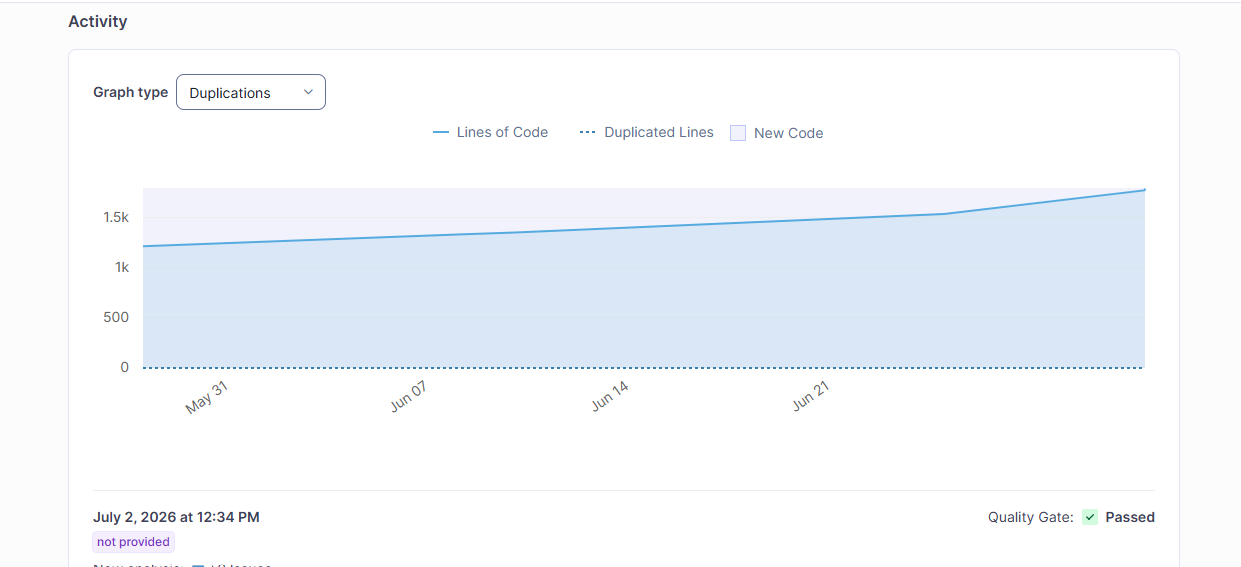
\includegraphics[width=1\textwidth]{images/SonarQube/SonarQubeDuplications.png}
    \caption{SonarQube Report - Indice di duplicazione}
    \label{fig:indiceDiDuplicazioneSQ}
\end{figure}
Come illustrato dal grafico, nel progetto non vi sono righe duplicate. L'assenza di codice ripetuto riflette un'architettura software efficiente, che previene l'aumento ingiustificato della complessità e garantisce un'ottima manutenibilità a lungo termine.


\paragraph{Indice degli Errori} -
\begin{figure}[H]
    \centering
    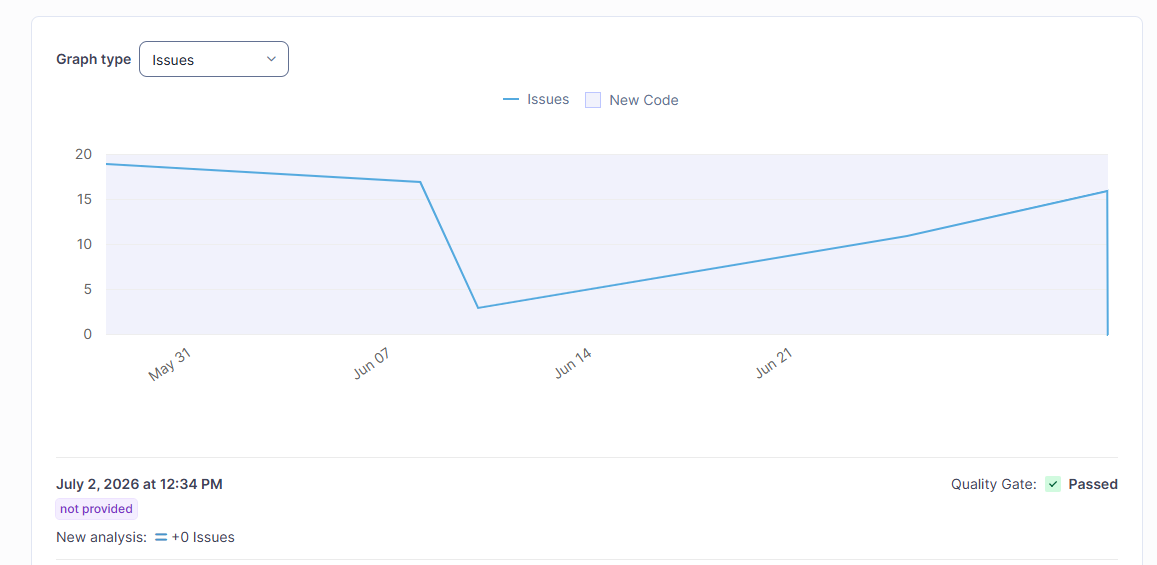
\includegraphics[width=1\textwidth]{images/SonarQube/SonarQubeIssues.png}
    \caption{SonarQube Report - Indice degli Errori}
    \label{fig:indiceErroriSQ}
\end{figure}
Come illustrato dal grafico, all'inizio dello sviluppo sono stati trovati 20 errori. Il nuovo codice ne ha generato altri 15, ma alla fine dello sviluppo sono stati completamente azzerati. Ciò indica un processo di miglioramento continuo della qualità del codice, con un’attenta risoluzione dei problemi rilevati durante l’analisi.

\paragraph{Report di qualità Overall} -
\begin{figure}[H]
    \centering
    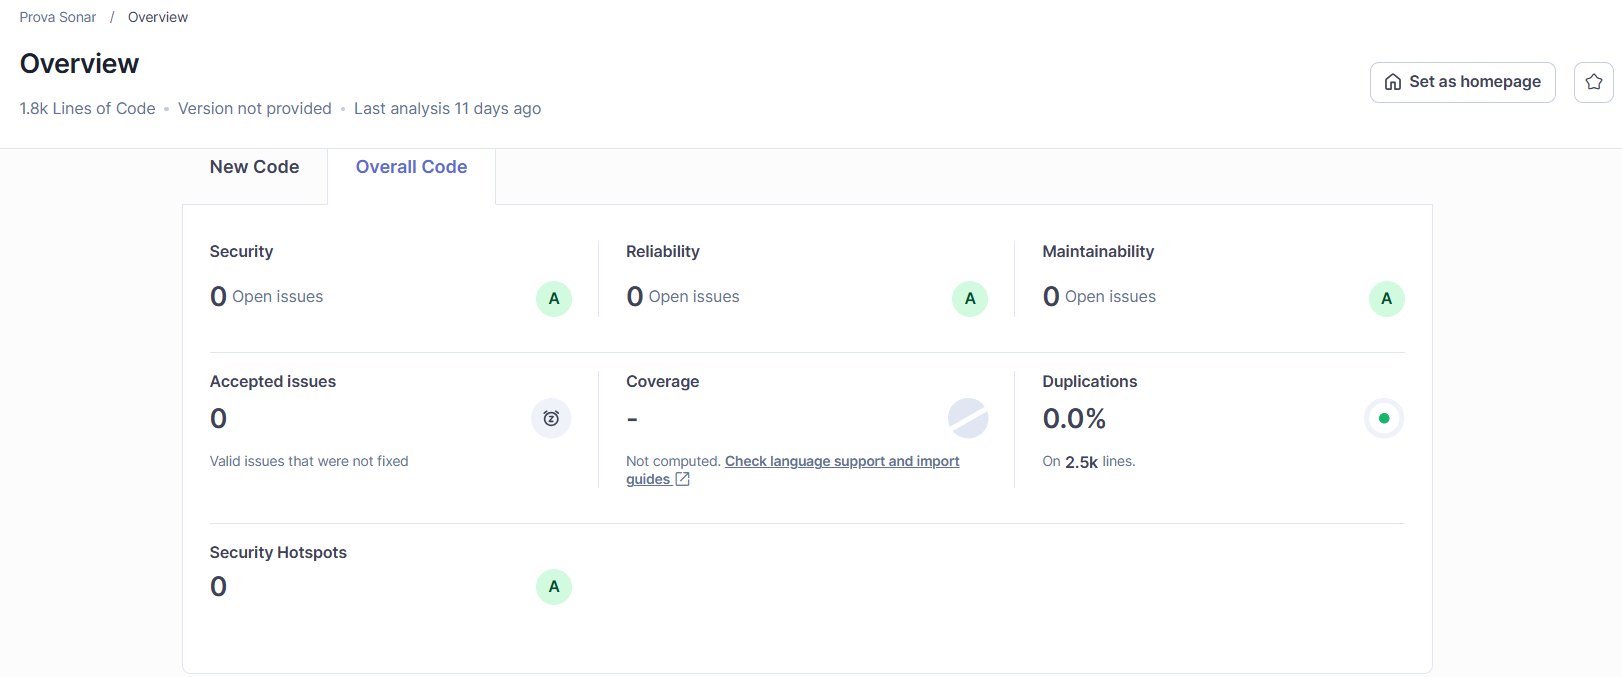
\includegraphics[width=1\textwidth]{images/SonarQube/SonarQubeReportOverall.png}
    \caption{SonarQube Report - Report Overall codice}
    \label{fig:reportOverallSQ}
\end{figure}

\paragraph{Report di qualità NewCode} -
\begin{figure}[H]
    \centering
    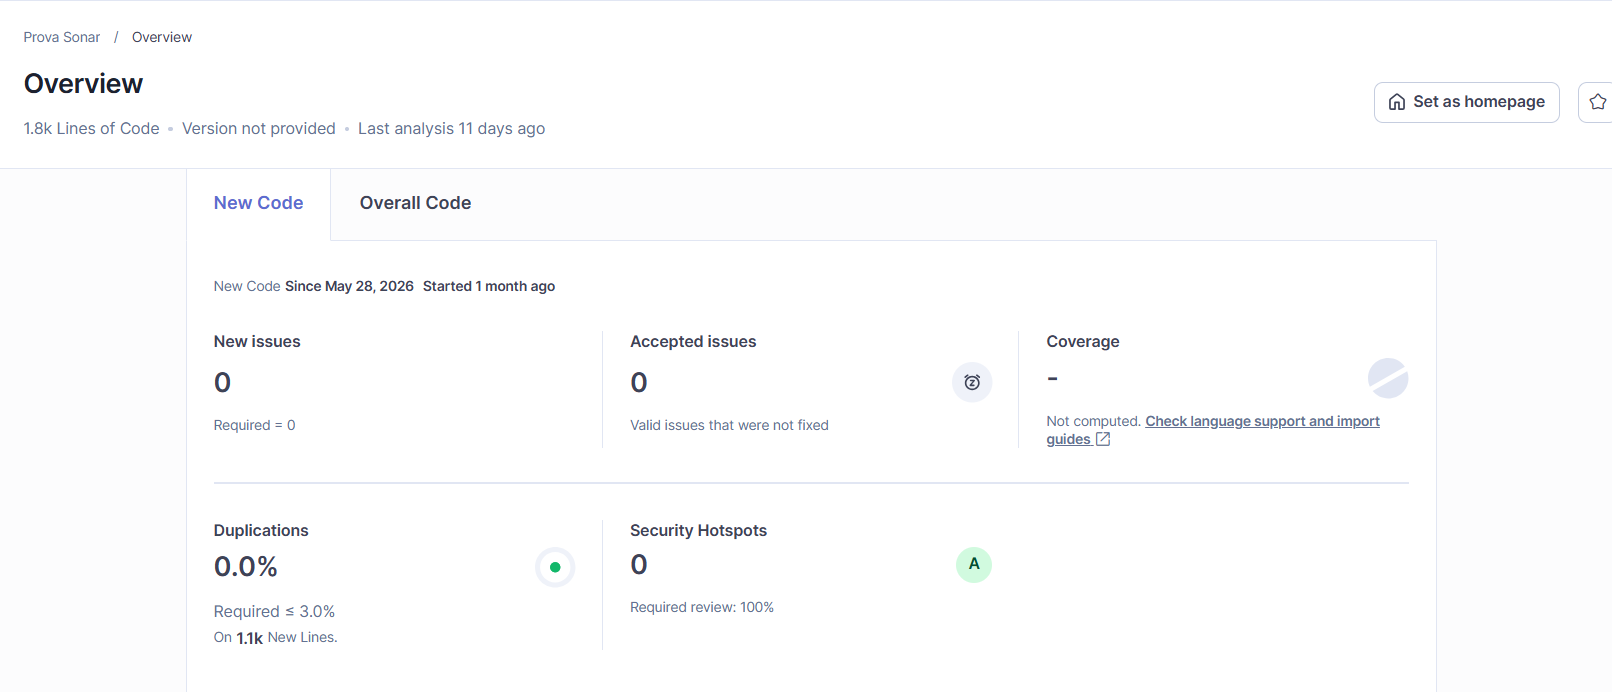
\includegraphics[width=1\textwidth]{images/SonarQube/SonarQubeReportNewCode.png}
    \caption{SonarQube Report - Report NewCode}
    \label{fig:reportNewCodeSQ}
\end{figure}



\printindex


\end{document}